% options:
% thesis=B bachelor's thesis
% thesis=M master's thesis
% czech thesis in Czech language
% slovak thesis in Slovak language
% english thesis in English language
% hidelinks remove colour boxes around hyperlinks

\documentclass[thesis=M,czech]{FITthesis}[2012/06/26]

\usepackage[utf8]{inputenc} % LaTeX source encoded as UTF-8
\usepackage{float}
% \usepackage{amsmath} %advanced maths
% \usepackage{amssymb} %additional math symbols
\usepackage{subfig,graphicx}
\usepackage{array}
\usepackage{color}
\usepackage{makecell}

\usepackage{dirtree} %directory tree visualisation

\usepackage{hyperref} %todo přidat do normální hlavičky %
\usepackage{longtable}

% % list of acronyms
% \usepackage[acronym,nonumberlist,toc,numberedsection=autolabel]{glossaries}
% \iflanguage{czech}{\renewcommand*{\acronymname}{Seznam pou{\v z}it{\' y}ch zkratek}}{}
% \makeglossaries

\newcommand{\tg}{\mathop{\mathrm{tg}}} %cesky tangens
\newcommand{\cotg}{\mathop{\mathrm{cotg}}} %cesky cotangens
\newcommand{\ptheory}{$\Psi$-theory }

% % % % % % % % % % % % % % % % % % % % % % % % % % % % % % 
% ODTUD DAL VSE ZMENTE
% % % % % % % % % % % % % % % % % % % % % % % % % % % % % % 

\department{Katedra softwarového inženýrství}
\title{Možnosti využití metodiky DEMO pro tvorbu BPMN modelů}
\authorGN{Štěpán} %(křestní) jméno (jména) autora
\authorFN{Heller} %příjmení autora
\authorWithDegrees{Bc. Štěpán Heller} %jméno autora včetně současných akademických titulů
\supervisor{Ing. Pavel Náplava}
\acknowledgements{Rád bych poděkoval mému vedoucímu Ing. Pavlu Náplavovi za cenné rady v průběhu tvorby práce a také Stevenu Van Kervelovi ze společnosti Formetis, který byl velkým přínosem pro vznik této práce.}
\abstractCS{V~několika větách shrňte obsah a přínos této práce v~češtině. Po přečtení abstraktu by se čtenář měl mít čtenář dost informací pro rozhodnutí, zda chce Vaši práci číst.}
\abstractEN{Sem doplňte ekvivalent abstraktu Vaší práce v~angličtině.}
\placeForDeclarationOfAuthenticity{V~Praze}
\declarationOfAuthenticityOption{4} %volba Prohlášení (číslo 1-6)
\keywordsCS{DEMO, BPMN, Enterprise ontology, Business Process Management, Proces, Procesní model}
\keywordsEN{DEMO, BPMN, Enterprise ontology, Business Process Management, Process, Process Model}

\begin{document}

% \newacronym{CVUT}{{\v C}VUT}{{\v C}esk{\' e} vysok{\' e} u{\v c}en{\' i} technick{\' e} v Praze}
% \newacronym{FIT}{FIT}{Fakulta informa{\v c}n{\' i}ch technologi{\' i}}

\begin{introduction}
	Každá organizace (nezáleží zda firma, úřad nebo spolek) od určité velikosti začne řešit problémy s efektivitou a udržitelností růstu. Jedním z řešení, ať už k němu řídící pracovníci přistoupí vědomě či nevědomě, je nějaká forma \textit{procesního řízení}.

Procesní řízení, jehož základům se podrobně věnuje kapitola 1, ve své podstatě znamená standardizaci opakujících se postupů, jejich zaznamenání ve formě, která umožní pozdější analýzu a optimalizaci za účelem zvyšování efektivity jejich provádění a eliminaci chyb, které mohou vzniknout.

Přístupy, jak procesy zaznamenávat, analyzovat a optimalizovat se vyvíjí stejně jako se vyvíjí organizace, společnost, požadavky zákazníků a v neposlední řadě technologie. Od intuitivního zaznamenávání průběhu procesů pomocí \textit{vývojových diagramů}, které neumožňovaly nic jiného než prosté grafické znázornění posloupnosti aktivit, se vývoj posunul k automatizaci procesů pomocí výpočetních prostředků a analýze velkého množství dat o každém kroku analyzovaného procesu.

Tato práce se snaží přispět k tomu, aby bylo možné procesy zaznamenávat a analyzovat s větší mírou konzistence podle metody, jejíž návrh tato práce představuje v kapitole 5.

\subsection{Motivace}
V této práci jsou analyzovány dvě techniky použitelné k modelování podnikových procesů – DEMO a BPMN. BPMN je v současnosti zřejmě nejpoužívanější notací pro vizuální reprezentaci podnikových procesů. Její předností je zejména velká srozumitelnost pro business uživatele, kteří jsou dobře obeznámeni s vývojovými diagramy a jsou tak schopni číst i vytvářet diagramy v BPMN bez větších problémů. Slabinou BPMN je však absence jasných pravidel \textit{jak} diagramy vytvářet, \textit{které} části procesu v nich zaznamenávat a \textit{z čeho} se procesy vlastně skládají. Výsledkem jsou BPMN modely, které jsou často \textit{nekompletní}, \textit{nekonzistentní} a \textit{nejednoznačné}.

DEMO je metodologie založená na silném teoretickém základu, který se skládá především z \textit{Enterprise ontology} a \textit{\ptheory}. DEMO má jasná pravidla co v modelech zachycovat, jak při vytváření modelů postupovat a jak ověřit, zda jsou vzniklé modely korektní a správné. Metodologie DEMO zajišťuje, že pokud dodržíme veškeré postupy, které tato metodologie stanoví, tak nám při modelování stejného procesu musí na konci vždy vzniknout ten samý model. Tato jistota má zásadní pozitivní důsledky pro analýzu, sdílení i diskusi nad procesy v rámci organizace.

Tato práce si klade za cíl zkombinovat výhody obou technik, tedy dobrou srozumitelnost business uživateli na straně jedné a pevný teoretický základ na straně druhé, vyvinutím metody, která umožní vytvářet BPMN modely, které budou \textit{kompletní}, \textit{konzistentní} a \textit{jednoznačné}. V kombinaci s možnostmi automatizace by se mohlo jednat o krok dopředu v celé oblasti Business Process Managementu.

\subsection{Struktura práce}
Práce je rozdělena do šesti kapitol. V první jsou definovány základní pojmy, se kterými je ve zbytku textu pracováno a také je zde rozebrán vývoj přístupů k práci s podnikovými procesy. Druhá kapitola analyzuje nejpoužívanější techniky pro modelování podnikových procesů a srovnává jejich silné a slabé stránky. Třetí a čtvrtá kapitola rozebírají notaci BPMN, respektive metodologii DEMO do hloubky – jejich základní principy a postupy. V páté kapitole se nachází klíčová část této práce, kterou je jednak jednak návrh toho, jak vyjádřit klíčové prvky metodologie DEMO pomocí primitiv z notace BPMN a také návrh metody, která obsahuje sedm kroků dle kterých je možné vytvořit BPMN model procesu. Výsledný model by měl být \textit{kompletní}, \textit{konzistentní} a \textit{jednoznačný}. Závěrečná kapitola demonstruje navrženou metodu na konkrétním příkladu a diskutuje výsledky její aplikace.

\subsection{Překlad cizojazyčných termínů}
Při psaní textu se autor potýkal s problémem, že zejména v případě metodologie DEMO existuje jen mizivé množství textů v českém jazyce, které by popisovaly tuto metodologii. Základní termíny, kterými jsou označeny jednotlivé prvky metodologie, tak nemají český překlad. Autor se rozhodl toto řešit částečným překladem těch termínů, u kterých je přeložení přímočaré a jinak pracoval s původními anglickými výrazy. Při případné aktualizaci práce by bylo možné přeložit více termínů, pokud by se na českých ekvivalentech našla shoda v rámci české komunity DEMO.

\subsection{Klíčové zdroje}
Pro čerpání informací použil autor této diplomové práce několik desítek zdrojů, ale tři níže uvedené stojí za vypíchnutí a krátký komentář, neboť byly pro vznik této práce zásadní.

\subsubsection{Enterprise ontology – Jan L. G. Dietz}
Jan Dietz je tvůrcem metodologie DEMO a autorem celé řady publikací na téma fungování organizací, sociálních interakcích v nich, stejně jako na modelování jejich činnosti. Kniha \textit{Enterprise ontology – Theory and Metodology} podrobně popisuje všechny tyto fenomény stejně jako Enterprise ontology, \ptheory a celou metodologii DEMO.

\subsubsection{Enhancing the Formal Foundations of BPMN by Enterprise Ontology – Van Nuffel, Mulder, Van Kervel}
Tato publikace je jednou z mála, které se zabývají nějakým druhem kombinace DEMO a BPMN. V tomto případě se jedná zejména o analýzu již existujících BPMN modelů z hlediska požadavků na ontologickou kompletnost a konzistentnost. Tato práce zároveň obsahuje postup, jak zajistit úpravu těchto BPMN modelů tak, aby tyto požadavky splňovaly.

V této souvislosti by autor rád zmínil, že v rámci tvorby této diplomové práce navštívil jednoho z autorů této publikace Stevena Van Kervela a jeho tým ve společnosti Formetis, za účelem diskutování závěrů a přínosů práce. Tato návštěva byla pro vznik této diplomové práce velkým přínosem.

\subsubsection{Business Process Modeling and Simulation: DEMO, BORM and BPMN – Zuzana Vejražková}
Třetí publikací, která byla zásadní pro vznik této diplomové práce je diplomová práce Zuzany Vejražkové, která vznikla na Fakultě informačních technologií ČVUT. Tato práce se zabývá analýzou technik DEMO, BORM a BPMN s důrazem na simulaci podnikových procesů, která umožňuje jejich efektivnější analýzu.

Rozdíl mezi touto diplomovou prací a prací Zuzany Vejražkové je jednak ve volbě technik, které jsou zkombinovány (Zuzana Vejražková kombinuje DEMO s Petriho sítěmi, tato práce kombinuje DEMO a BPMN) a jednak v menším důrazu na simulaci a automatizaci, kterou autor této diplomové práce přenechává dalšímu výzkumu.
\end{introduction}

\chapter{Definice základních pojmů}
	\documentclass[]{article}
\usepackage[czech]{babel}
\usepackage[utf8]{inputenc}

\begin{document}

\title{Kapitola 1: Definice základních pojmů}
\author{Bc. Štěpán Heller}
\date{\today}
\maketitle

\section{Motivace k řízení podnikových procesů}
Každá firma, která se snaží efektivně řídit svůj chod a neustále se rozvíjet stále hledá nové a nové cesty, jak toho docílit. Takovými cestami může být uvádění nových produktů na trh, hledání nových trhů a příležitostí na nich, nabírání nových zaměstnanců, investice do propracovaného marketingu a mnoho dalších. Stále více firem ale v posledních několika dekádách obrací svou pozornost také dovnitř vlastní organizace. Hledají oblasti, kde je možné najít úspory nebo kde by bylo možné práci zefektivnit.

Aby bylo něco takového vůbec možné, musí mít manažeři a odpovědní vedoucí pracovníci především přehled o své organizaci a její hlubokou znalost. Pouze z takové hluboké znalosti pak mohou vzejít příležitosti k efektivnějšímu dosahování podnikových cílů.

Z toho důvodu firmy a organizace hledají cesty, jak lépe pochopit a následně standardizovat \textit{procesy} v rámci vlastního podniku, které ve svém souhrnu nejsou nic jiného než soubor postupů, kterými podnik nebo organizace dosahuje svých cílů. O tom, kterak takové procesy pozorovat, standardizovat a řídit, byla napsána celá řada publikací a je nezbytné mít na zřeteli, že se jednotlivé přístupy od sebe více či méně odlišují. 

Ačkoliv akademici i odpovědní lidé z prostředí samotných firem a organizací se často přou, který z přístupů je lepší, zůstává bez nejmenších pochyb, že adoptování jakéhokoliv přístupu vedoucího k lepšímu porozumění chodu vlastní organizace je lepší, než nahodilý přístup k řízení společnosti, kdy jsou změny vykonávany ad hoc a jakékoliv plánování do budoucna je tak velmi obtížné. Pochopení vlastní organizace je jedním (nikoli jediným) ze základních předpokladů pro její dlouhodbě udržitelný rozvoj a právě k tomu jsou procesy a procesní řízení široce akceptovaným přístupem.

The main objective of process management is to find the most efficient and effective way to transform customer requirements into customer satisfaction.

\section{Definice základních pojmů}
V rámci této sekce jsou definovány základní pojmy, jejichž znalost a plné porozumění je nezbytné pro orientaci v obsahu dalších kapitol.
\subsection{Podnikový proces}
V nadsázce řečeno definic pojmu \textit{proces} existuje tolik, kolik existuje publikací, které jsou jim věnovány. Intuitivně si člověk s těmito definicemi neseznámený představí určitou po sobě jdoucí posloupnost operací na jejichž konci může být nějaký výsledek.

Norma EN ISO 9000:2000 definuje pojem proces následovně: \cite{iso_9000}

\begin{quote}
Proces je soubor vzájemně působících nebo vzájemně souvisejících činností, které přeměňují vstupy na výstupy.
\footnote{Set of interrelated or interacting activities which transforms inputs into outputs.}
\end{quote}

O něco podrobnější definici můžeme najít v \cite{Weske2007}:

\begin{quote}
Podnikový proces se skládá ze souboru činností, které jsou prováděny koordinovaně v organizačním a technickém prostředí. Tyto činnosti společně plní podnikový cíl. Každý podnikový proces je prováděn jednou organizací, ale může vzájemně působit s procesy prováděnými jinými organizacemi.
\footnote{A business process consists of a set of activities that are performed in coordination in an organizational and technical environment. These activities jointly realize a business goal. Each business process is enacted by a single organization, but it may interact with business processes performed by other organizations. \cite{Weske2007}}
\end{quote}

I když je možné proces vnímat jako izolovanou jednotku, je na tomto místě dobré si uvědomit, že proces v organizaci je velmi často výstupem jiného procesu. Mezi hlavní atributy procesu patří: \cite{Bandor2007}

\begin{itemize}
\item \textit{Název}, který proces identifikuje.
\item \textit{Účel}, pro který je proces prováděn.
\item \textit{Vlastník}, který je za proces zodpovědný (osoba nebo složka v organizaci).
\item \textit{Specifikace vstupů}. Věci, které jsou potřebné k provádění procesu.
\item \textit{Specifikace výstupů}. Věci, které jsou vytvořeny v průběhu provádění procesu.
\item \textit{Vstupní a výstupní podmínky}, které musí být splněny při spuštění a ukočení procesu.
\item \textit{Činnosti} definují jednotlivé kroky (operace) při provádění procesu.
\item \textit{Role a zodpovědnosti} definují, kdo je zodpovědný za provedení konkrétní činnosti.
\end{itemize}

\subsubsection{Produkt}
Dle \cite{iso_9000} je produkt definován jednoduše jako výsledek procesu. Produkt se dále může skládat z dalších produktů, které jsou výsledkem činnosti jiných procesů.

\subsubsection{Procedura}
Proceduru definujeme dle \cite{iso_9000} jako \textit{\uv{určený způsob, jak vykonat činnost nebo proces}}.
\footnote{Specified way to carry out an activity or a process.\cite{iso_9000}}

Pro správné pochopení rozdílu mezi procesem a procedurou je třeba si uvědomit, že proces nám říká \uv{co je potřeba udělat, a které role jsou zastoupeny} a procedura \uv{jak to udělat} a většinou se týká pouze jedné role. \cite{Bandor2007}


\subsection{Řízení podnikových procesů}
The main objective of process management is to find the most efficient and effective way to transform customer requirements into customer satisfaction. \cite{Jedlitschka2010}
\subsection{Business Process Management System}
\subsection{Capability Maturity Model}
\subsection{Business Process Model}
\subsection{Business Process Lifecycle}
\subsection{Classification of Business Processes}

\section{Vývoj přístupů k řízení podnikových procesů}

\bibliographystyle{plain}
\bibliography{Bibliography}

\end{document}

\chapter{Techniky modelování podnikových procesů}
	\documentclass[]{article}
\usepackage[czech]{babel}
\usepackage[utf8]{inputenc}
\usepackage{float}
\usepackage{graphicx}


\begin{document}

\title{Kapitola 2: Techniky modelování podnikových procesů}
\author{Bc. Štěpán Heller}
\date{\today}
\maketitle

\section{Procesní model a důvody pro jeho tvorbu}
Ať už člověk vytváří jakýkoliv model, jeho cílem je zachytit nějaký jev, který je potřeba kvůli své komplexnosti zobrazit zjednodušenou vizuální formou, která bude pochopitelná i pro jiné lidi než je sám tvůrce modelu. Umět jev zachytit ve formě modelu je jedním z prvních kroků na cestě k tomu tento jev upravovat.

Přeneseno do světa podnikových procesů je to velmi podobné. Jedním z hlavních důvodů, proč organizace přistupují k práci s BPM je potřeba procesy upravovat a zejména optimalizovat. Aby to bylo možné, je potřeba nejdřív stanovit metriky a tyto metriky být pak schopen měřit. Základem pro všechny tyto kroky je ale korektní procesní model, který proces věrně popisuje.

\subsection{Definice procesního modelu}
Základní definice procesního modelu podle 
\begin{quote}
Procesní model je konceptualizací podnikového procesu v organizaci.
\footnote{Process model is a conceptualization of the (business) process in an enterprise. \cite{Dietz2006}}
\end{quote}
Čtenářsky přístupnější definici pak nabízí \cite{Recker2009}
\begin{quote}
Procesní model popisuje, většinou grafickou formou aktivity, události, jejich pořadí a propojení, které utváří podnikový proces.
\footnote{Process model describe, typically in a graphical way, the activities, events and control flow logic that constitues a business process.}
\end{quote}

\section{Základní techniky}
V této sekci si popíšeme populární techniky pro tvorbu procesních modelů.
\subsection{Vývojový diagram (flowchart)}
Vývojový diagram je pravděpodobně nejpopulárnější technikou pro modelování podnikových procesů. Vděčí za to zejména své jednoduchosti, dostupnosti mnoha nástrojů, které tuto techniku podporují a také její velké srozumitelnosti, která jí činá velmi snadno uchopitelnou i pro uživatele v organizaci, kteří nejsou příliš obeznámeni s problematikou modelování podnikových procesů.

\subsubsection{Základní pravidla}
Vývojové diagramy se skládají z několika málo základních symbolů. Tyto symboly se nazývají: \cite{Chytil2005}

\begin{itemize}
\item Startovací a ukončovací symboly – používají se pro vyznačení začátku a konce procesu
\item Šipky – zobrazují tzv. \uv{řídící tok}, tedy přechod v čase mezi jednotlivými symboly
\item Dílčí kroky procesu – jsou reprezantovány obdelníkem.
\item Podprogramy – zobrazeny obdelníkem se svislými čarami po stranách. Používají se pro zobrazení skupiny kroků procesu pomocí jediného symbolu.
\item Vstupy a výstupy – zobrazují tok informací směrem dovnitř i vně procesu, Pro jejich reprezentaci se používají lichoběžníky respektive rovnoběžníky.
\item Podmíněný cyklus – zobrazuje událost opakující dokud je splněna jasně definovaná podmínka. Zobrazuje se pomocí šestiúhelníku.
\item Podmíněný výraz – kosočtvercem je symbolizováno rozhodnutí a určuje tedy místo, kde dochází k větvení procesu.
\item Spojovací symbol – inverzním symbolem ke kosočtverci je ve vývojovém diagramu kruh, který se používá ke spojení více toků do jednoho.
\end{itemize}

\begin{figure}[H]\centering %todo překreslit obrázek%
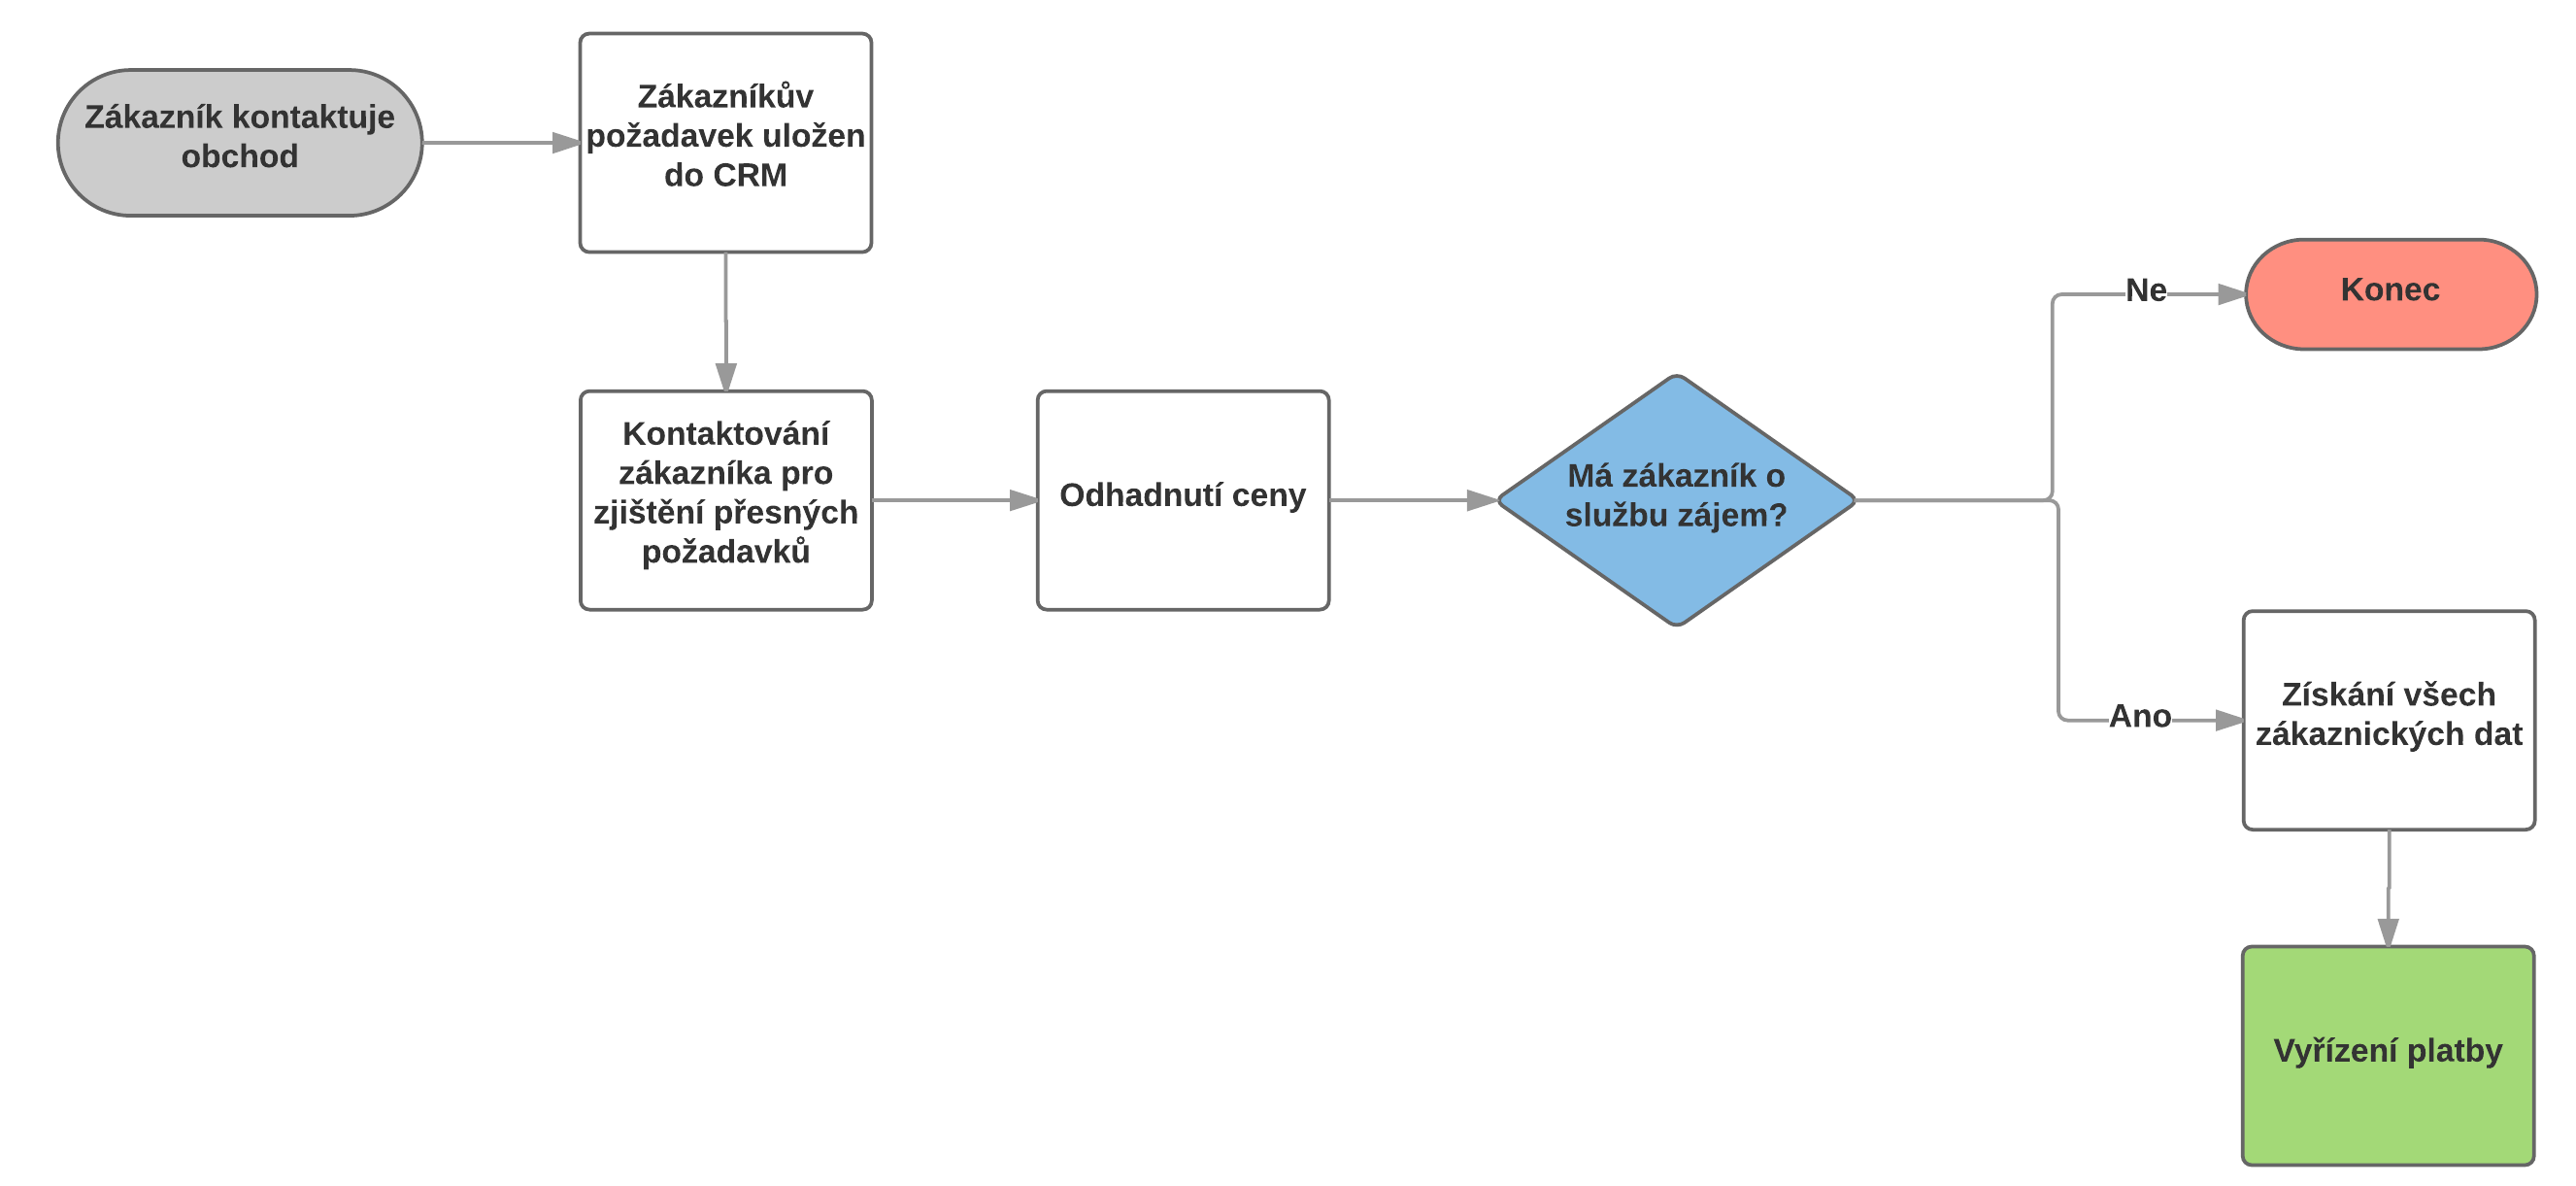
\includegraphics[width=1.0\textwidth]{obrazky/flowchart}
\caption{Nákupní proces pomocí vývojového diagramu}
\label{fig:Flowchart}
\end{figure}

\subsubsection{Výhody a nevýhody}
Nespornou výhodou vývojových diagramů je právě jejich přístupnost pro uživatele a velmi strmá křivka učení, což dělá z této techniky první volbu pro případy, kdy je potřeba velmi rychle vymodelovat nějaký proces a organizace nemá zavedeny sofistikovanější metody BPM. Vývojové diagramy umožňují efektivnější komunikaci o problému v rámci týmu. 

Největší přednost vývojových diagramů je zároveň jejich největší slabinou. Právě přílišná jednoduchost této techniky dělá z modelování komplexnějších procesů poměrně komplikovanou a nepřehlednou záležitostí. Ve vývojových diagramech je také složitější modelovat některé jevy, jako například tzv. \uv{unhappy paths} a další nestandardní události, která však v životě procesů nastávají poměrně běžně. U vývojových diagramů je také obtížné dělat změny, protože to často vyžaduje kompletní překreslení celého diagramu.

\subsubsection{Použití}
Vývojové diagramy mají mnoho využití. Hodí se například pro komunikaci mezi organizací a jejími externími zákazníky, protože se dá předpokládat, že se s vývojovými diagrami už v minulosti setkali a budou jim tedy rozumět. Vhodné je také použít vývojový diagram v dokumentaci k softwaru nebo jinému systému, kterou budou číst různorodé skupiny uživatelů.

\subsection{BPMN}
BPMN nebo rozepsaně Business Process Modelling Notation je v současnosti de facto standardem na poli modelování podnikových procesů. Jeho využití je široké od IT přes obchod až například po komplexní dopravní systémy. Za svou popularitu vděčí zejména kombinaci dvou věcí, z nichž jedna je stále poměrně jednoduchá notace, která neobsahuje přehršel symbolů.

S trochou nadsázky by se dalo říct, že BPMN je vlastně rozšířením vývojového diagramu. Je určitě pravdou, že se BPMN touto jednoduchou technikou v mnohém inspirovalo a na jejích základech postavilo notaci, která umožňuje poměrně jednoduše modelovat i komplexní podnikové procesy a zároveň si stále uchovává dobrou srozumitelnost pro uživatele.

\subsubsection{Základní pravidla}
Jelikož se BPMN budeme podrobně věnovat v kapitole 3 %todo odkaz%
nemá smysl na tomto místě zacházet do přílišných detailů. Zatím si vystačíme s tím, že v BPMN jsou zásadními objekty aktivity, události, brány, počáteční a koncové symboly a \uv{šipky} neboli symboly řízení toku procesu. Vzhledově se příliš neliší od korespundujících symbolů ve vývojovém diagramu.

\begin{figure}[H]\centering %todo překreslit obrázek%
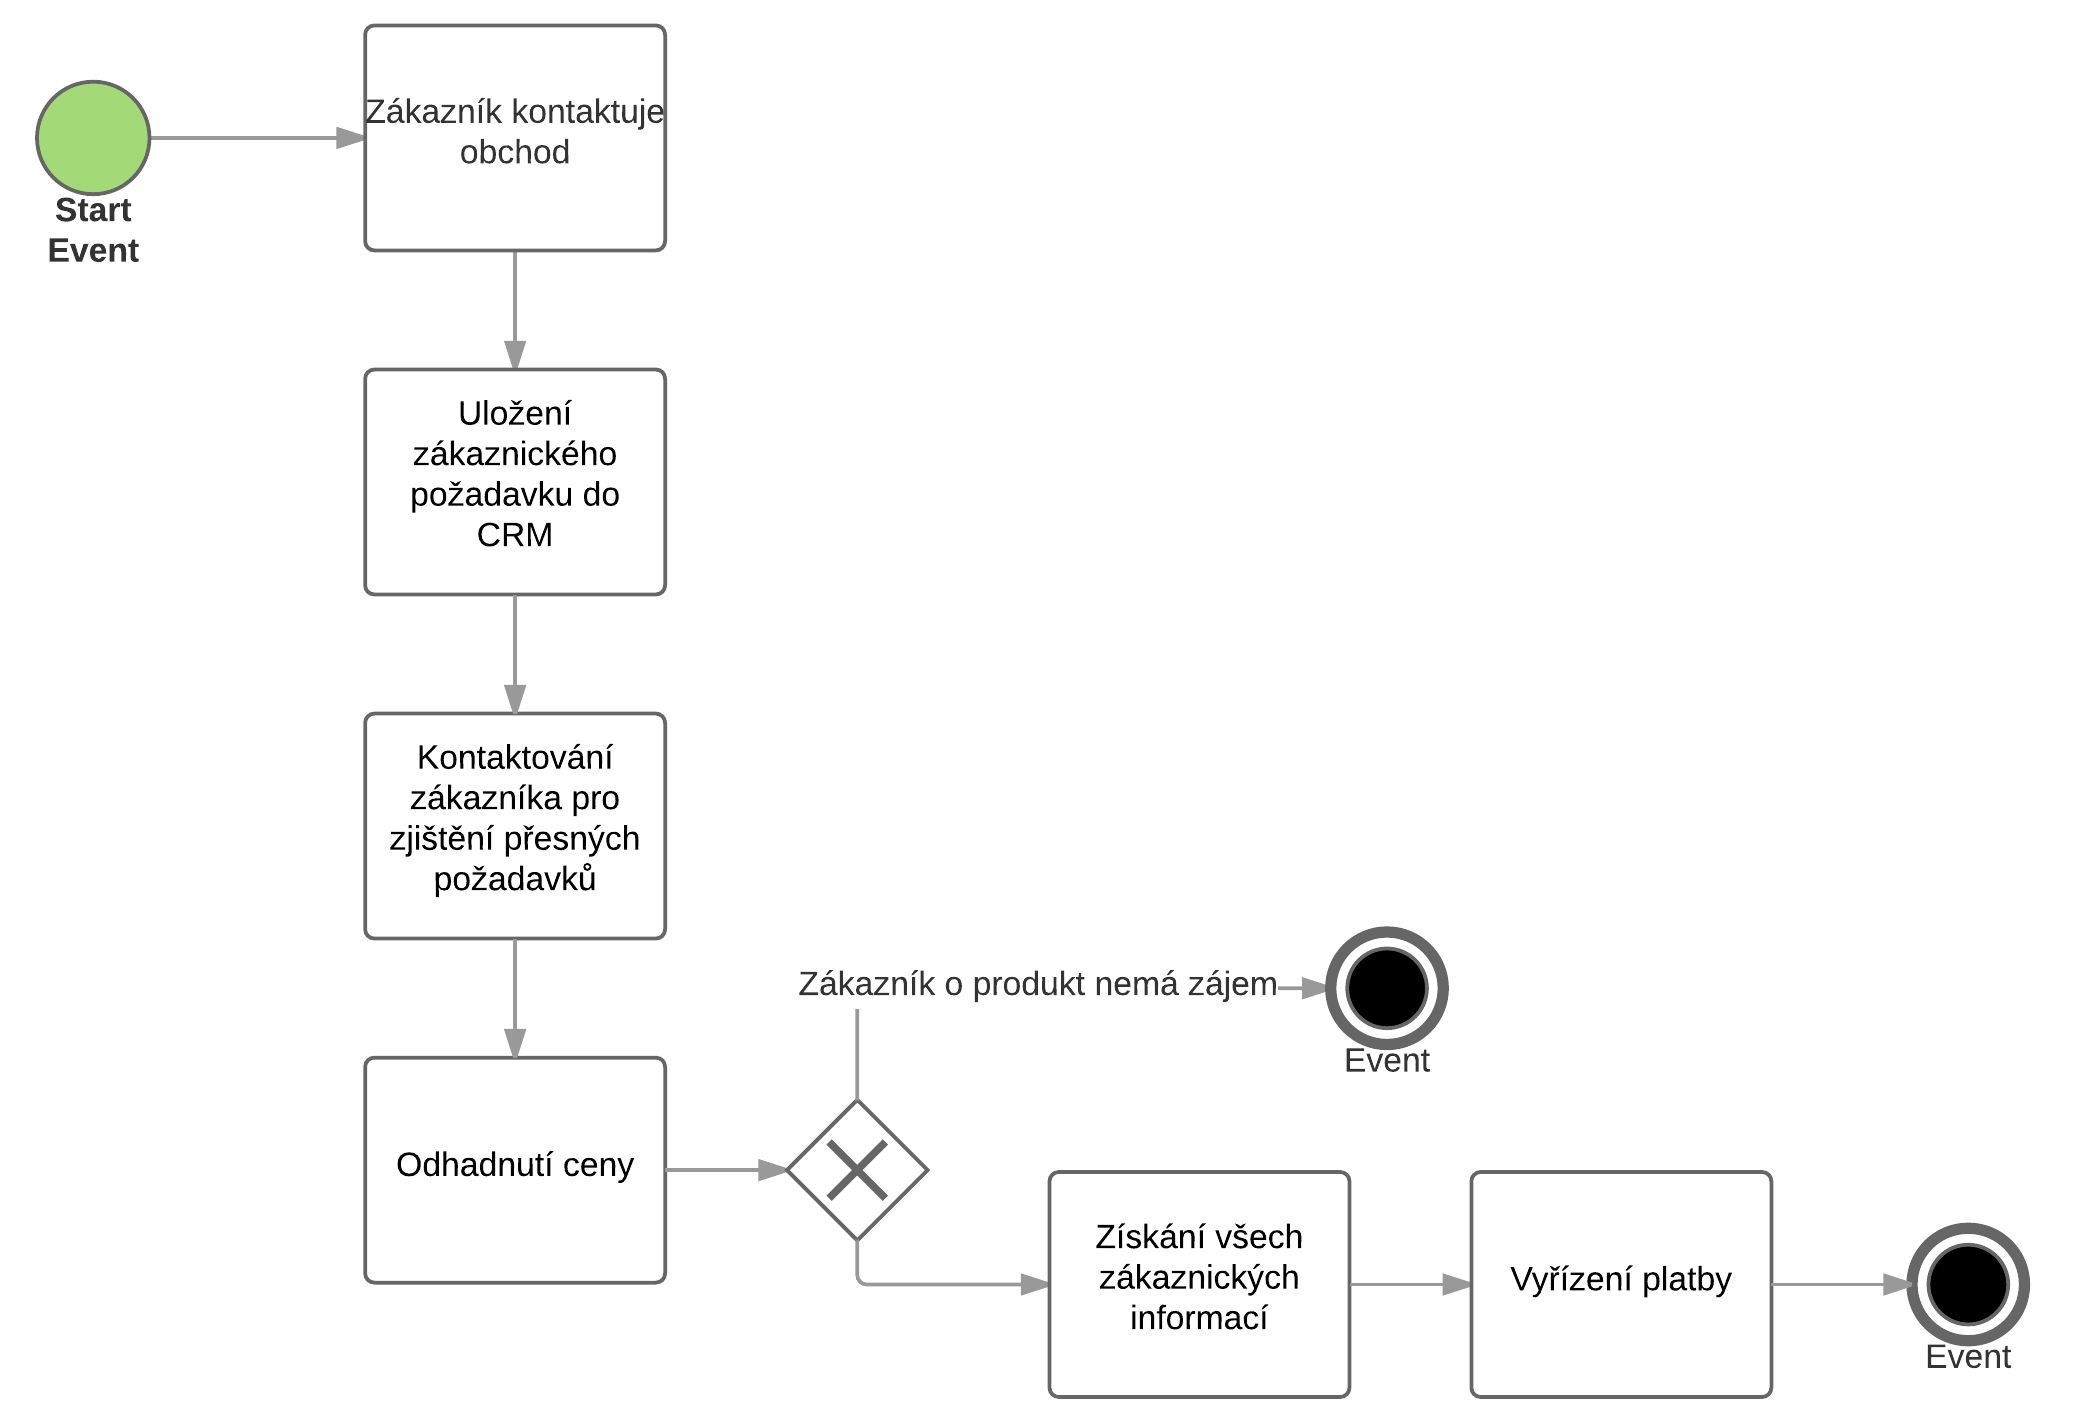
\includegraphics[width=1.0\textwidth]{obrazky/bpmn_nakupniproces}
\caption{Nákupní proces pomocí BPMN}
\label{fig:BPMN_nakupniproces}
\end{figure}

\subsubsection{Výhody a nevýhody}
Mezi hlavní výhody BPMN určitě můžeme zařadit fakt, že BPMN je standard, tedy je přesně definované jak a kdy, které symboly používat. O BPMN se stárá organizace OMG (Object Management Group) a kontinuálně pracuje na jeho rozvoji. Díky širokému rozšíření BPMN existuje na trhu velké množství placených i neplacených nástrojů, které umožňují modelování podnikových procesů pomocí této notace.

Další neoddiskutovatelnou předností je srozumitelnost notace, která je vysoká právě díky své podobnosti k vývojovým diagramům. Bez nutnosti zdlouhavého studia dokumentace je BPMN modelu schopen porozumět člověk z managementu společnosti a stejně tak i softwarový inženýr nebo vývojář. Právě pro ty ukrývá BPMN další výhodu a tou je poměrně přímočará převoditelnost BPMN modelů do strojově čitelných formátů, jako je jazyk XML nebo na něm založený jazyk BPEL. %todo ověřit%

Ačkoliv je používání notace BPMN definované v dokumentaci, reálné procesy v organizacích mohou být obtížně modelovatelné bez hluboké znalosti BPMN a může tedy docházet k vytváření nekorektních modelů nebo více různých modelů toho samého jevu. Dalším problémem dle \cite{Polancic2014} je, že někteří výrobci softwaru pro modelování v BPMN si tento standard ohýbají podle sebe nebo ho \uv{obohacují} o vlastní \uv{vylepšení}, která pak dělají takto vytvořené modely obtížně přenositelnými.

\subsubsection{Použití}
Organizace OMG, která BPMN nyní spravuje, uvádí jako hlavní poslání BPMN přenositelnost procesních modelů vytvořených v této notaci nezávisle na tvůrcích konkrétního modelovacího nástroje. BPMN je vhodné pro modelování podnikových procesů v celé jejich šíři.

\subsection{BPEL}
BPEL neboli Business Process Execution Langauge (a správněji WS-BPEL Web Service Business Process Execution Language) je v našem výčtu jedinou technikou pro modelování podnikových procesů, který nemá grafickou reprezentaci. Je to totiž jazyk. Své využití nachází zejména při automatizaci podnikových procesů. BPEL je založen na XML a v podstatě standradizuje definici podnikových procesů právě pomocí XML. \cite{BPELcz}

\subsection{UML}
UML neboli Unified Modeling Language je velmi populární grafický jazyk, zvláště v oblasti IT a vývoje softwarových systémů. Jak píše \cite{Eriksson} právě s tímhle cílem bylo UML původně také vytvořeno. Jenže jeho popularita se rychle rozšířila i do světa byznysu a UML přestalo dostačovat potřebám svých uživatelů. Proto bylo postupně rozšiřováno o další aspekty, které pokrývaly modelování podnikových procesů v celé jejich šíři.

UML obsahuje standardizovaný mechanismus jak jazyk rozšiřovat tak, aby jeho obecné principy mohly být doplněny o další vyhovující specifickému účelu, jako je například právě modelování podnikových procesů. Proto byl již v době vzniku UML vytvořen standardní profil pro modelování podnikového procesu \cite{Repa2007}. Tento profil pracuje zejména s Diagramem tříd a s Diagramem Use-Case. Diagram Use-Case je v tomto profilu používán pro zobrazení podnikových procesů a jejich interakce s aktéry a zákazníky. Oproti tomu Diagram tříd se používá spíše k zobrazení vnitřní struktury popisované organizace. Faktem je, že se standardní profil pro modelování podnikového procesu v praxi příliš neujal, snad kvůli své přílišné snaze podnikové procesy přiblížit k IT a informančím systémům \cite{Repa2007}.

UML se přesto pro modelování podnikových procesů používá a to buď v neformální podobě, kdy je organizacemi používán především Diagram aktivit, který je pro modelování podnikových procesů vhodný. Activity Diagram totiž umožňuje sekvenční i paralelní zobrazování aktivit a objekty na vstupu i výstupu procesu a také závislosti mezi jednotlivými aktivitami.

Pro větší přenositelnost a potřeby standardizace UML jazyka pro modelování podnikových procesů však vznikla celá řada rozšíření třetích stran. Mezi nejpoužívanější pak patří rozšíření podle H. Erikssona. \cite{Repa2007,Eriksson2000}. 

\begin{quote}
Erikssonův přístup je nejenom rozšířením UML, ale do značné míry plnohodnotnou metodou modelování procesů – určuje sadu modelů a diagramů, postavených vesměs na standardních diagramech UML. \cite{Repa2007}
\end{quote}

Erikssonovo rozšíření obsahuje více různých diagramů, přičemž pro potřeby samotného modelování podnikového proceus je nejzásadnější Diagram procesů, který je rozšířením právě již výše zmíněného Diagramu aktivit. Právě tomu se tedy budeme v této kapitole věnovat.

\subsubsection{Základní pravidla}
Diagram aktivit obsahuje několik základních prvků: \cite{UMLActivity}

\begin{itemize}
\item Aktivita – proces, který modeluje
\item Akce – jedná se o konkrétní činnost v rámci aktivity
\item Zahájení a ukončení – Počáteční a koncový uzel
\item Řídící tok – určuje pořadí vykonávání jednotlivých kroků aktivity, znázorněné pomocí šipek
\item Rozhodnutí – rozvětvení procesu na základě určité podmínky
\item Spojení – spojuje více toků do jednoho
\item Rozdělovník a spojovník – pro provádění více akcí paralelně se používá rozdělovník a spojovník
\item Příchozí událost – používá se, pokud je k provedení některých kroků potřeba akce zvenčí
\item Spuštění události – používá se, pokud je potřeba znázornit akci, která spouští jiný proces nebo akci
\end{itemize}

\begin{figure}[H]\centering
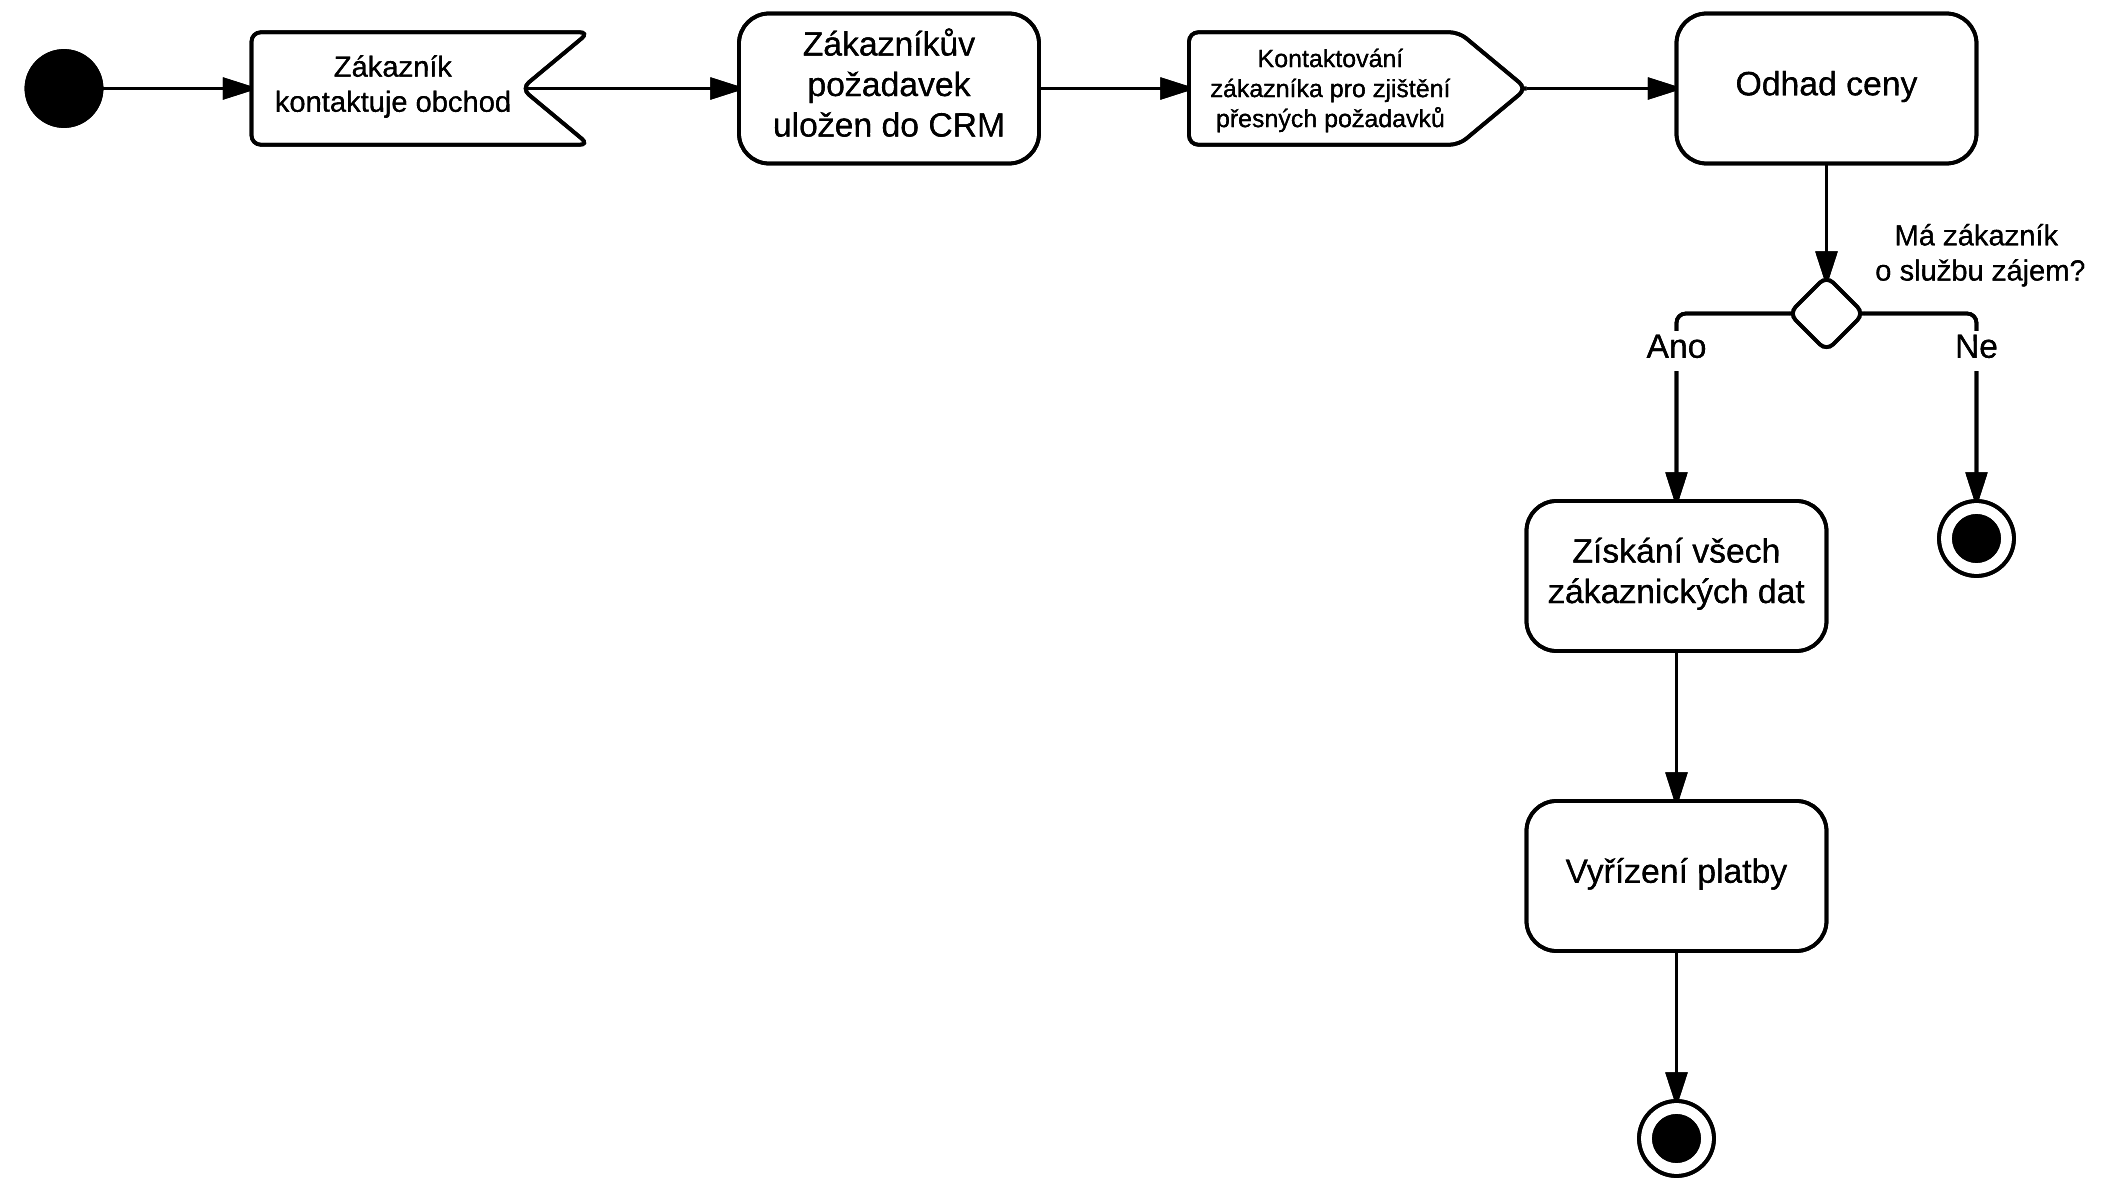
\includegraphics[width=1.0\textwidth]{obrazky/uml_nakupniproces}
\caption{Nákupní proces pomocí UML}
\label{fig:UML_nakupniproces}
\end{figure}

\subsubsection{Výhody a nevýhody}
Mezi výhody UML můžeme určitě zařadit velkou rozšířenost tohoto jazyka a s tím spojenou i velkou dostupnost nástrojů umožňujícících modelování v UML, literatury i komunit, kde je možno hledat pomoc či radu.

Jako nevýhodu lze určitě uvést faktickou neexistenci standardu pro modelování podnikových procesů v UML. Standardní profil pro modelování podnikového procesu, který UML obsahuje, se příliš nepoužívá a od verze UML 2.0 už dokonce není součástí množiny standardních profilů. \cite{Repa2007} Existují sice další rozšíření, ale ty nejsou standardem, což snižuje možnost jejich přenositelnosti i udržitelnosti do budoucna. UML je přecijen jazyk stále velmi blízký vývoji softwaru a modelování podnikových procesů spíše umožňuje, než podporuje.

\subsubsection{Použití}
Jak už bylo řečeno výše, UML nachází uplatnění v mnoha oborech lidské činnosti, ale prosadilo se zejména v IT a tvorbě softwaru. Některé nástroje, které umožňují modelování v UML dokonce nabízí možnost z UML modelu exportovat přímo zdrojový kód například pro tvorbu databáze.

Jelikož UML obsahuje různé druhy modelů, dostává tím celý jazyk další možnosti využití i mimo IT. Síla UML je v zachycení struktury jevu a již tolik nezáleží na tom, jestli se jedná o databázi nebo organizační strukturu podniku. Například Use-Case diagram najde využití nejen při modelování chování člověka při interakci se softwarem, ale například také obsluhy zákazníka v bance apod. 

UML je tak mimo jiné využíváno v IT, bankovnictví, telekomunikacích, zdravotnictví nebo v obranném průmyslu.

\subsection{DEMO}
DEMO neboli Design \& Engineering Methodology for Organizations je metodologie se silným teoretickým základem určená k modelování, analýze a grafickému zobrazení podnikových procesů. Za jejím vznikem stojí zejména Jan Dietz. DEMO obsahuje 4 modely, každý pro jiný účel a jiný pohed na proces.

\begin{quote}
Tímto způsobem jsme schopni rozmotat uzel,  který dnešní organizace připomínají, odstranit chyby v jejich návrhu a přitom zajistit, aby vše fungovalo. Stejně jako by inženýr opravil most, letadlo nebo počítač. \cite{DEMO_web}
\footnote{This way we can untangle the complex knot that organizations have become, fix the constructional mistakes, and put everything back together. Just like an engineer would repair a bridge, airplane or computer. \cite{DEMO_web}}
\end{quote}

Fundementální vlastnosti DEMO modelu dle \cite{Dietz2006} jsou:

\begin{itemize}
\item ucelený,
\item konzistentní,
\item úplný,
\item výstižný,
\item obsahovat jen nezbytné množství informací.
\end{itemize}

Zjednodušeně řečeno, důvodem pro vytvoření této metodologie byla narůstající nevhodnost jiných metodologií, notací a jazyků obvykle používaných k modelování podnikových procesů. %todo zdroj?% 
Modely vytvořené v těchto nástrojích jsou totiž většinou příliš podrobné a příliš technicky zaměřené, takže stěžují pohled na organizaci z vrchu, pohled jen na to důležité, co se v ní odehrává.

DEMO je naopak postaveno na modelování podnikových procesů pomocí ontologií, což znamená, že je zachyceno jen jádro problému, které většinou tvoří komunikace mezi lidmi. DEMO má silný teoretický základ v teorii PSI, o které si více řekneme v kapitole 4. %todo odkaz%

\subsubsection{Základní pravidla}
Detailnímu popisu modelování v DEMO se věnuje kapitola 4, takže na tomto místě zmíním jen základní věci. Kompletní model organizace (tzv. essential model) se skládá ze 4 různých modelů: \cite{Vejrazkova2012}

\begin{enumerate}
\item Construction Model (CM)
\item Process Model (PM)
\item Action Model (AM)
\item State Model (SM)
\end{enumerate}

Jedním z nejdůležitějších aspektů metodologie DEMO je tzv. \uv{transaction pattern}, který dává přesnou strukturu tomu, jak probíhají transakce (například objednávka). V DEMO se takové transakce skládají vždy ze stejných kroků a tudíž mají všechny stejnou strukturu, což zanechává malý prostor pro více interpretací stejné transakce.

Nejdůležitější aspekty v DEMO jsou 2:

\begin{enumerate}
\item Ontologická transakce
\item Actor role
\end{enumerate}

Podrobně budou tyto elementy rozebrány v kapitole 4. %todo odkaz°

%todo order process img%

\subsubsection{Výhody a nevýhody}
Mezi silné stránky metodologie DEMO určitě musíme zařadit jeho absolutní jednoznačnost. Zatímco u jiných nástrojů, jako je třeba vývojový diagram, ale i BPMN nebo UML, vzhledem k jejich poměrně vysoké úrovni detailu, může docházet k nejednoznačnostem, tj. že stejný jev je vymodelován různě. DEMO díky svým poměrně rigidním pravidlům a modelu postavenému na jasně strukturovaných transakcích dostáváme stejné modely pro stejné jevy, což je velmi pozitivní pro celkovou konzistenci BPM v organizaci a zároveň to usnadňuje analýzu a vylepšování procesů.

Jako hlavní přednost DEMO uvádí \cite{Barjis2011} schopnost modelů vytvořených pomocí této metodologie zachytit pouze základní podstatu každé organizace a schopnost modely abstrahovat od technických detailů, které jsou pro účely modelování organizací podružné.

Jako nevýhodu celé metodologie je určitě nutné označit poměrně dlouhou a pozvolnou křivku učení, která je v tomto případě dána 2 věcmi:

\begin{enumerate}
\item Široký teoretický základ, který sahá až do oblasti ontologie, filozofie a dalších oborů. I samotná metodologie má za sebou velmi robustní teorii, která není na první pohled zřejmá.
\item Narozdíl od vývojových diagramů nebo BPMN jsou modely vytvořené v DEMO pro člověka nezasvěceného do toho, jak DEMO funguje, prakticky nečitelné.
\end{enumerate}

Když by chtěla organizace začít používat DEMO pro modelování svých procesů, je nutné investovat čas i finanční prostředky do zasvěcení odpovědných lidí do metodologie a jejího používání, přičemž vycvičení lidí na potřebnou úroveň může být poměrně zdlouhavé. Právě toto by mohlo být jednou z hlavních překážek, které brání většímu rozšíření metodologie DEMO mimo akademickou půdu.

\subsubsection{Použití}
Tato část je založena zejména na \cite{Vejrazkova2012}, kde jsou uvedeny nejméně 3 možné způsoby, jak využít DEMO.

\begin{enumerate}
\item \textbf{Návrh a optimalizace organizací} – Díky přednostem metodologie DEMO, které jsou popsány výše, je možné se na organizaci podívat z ontologického hlediska, což umožňuje snáze pochopit, jak organizace skutečně funguje a je možné fungování jednotlivých procesů vylepšit a zefektivnit.
\item \textbf{Softwarová podpora organizace} – Jelikož velká část podnikových procesů je dnes podporována IT systémy. DEMO rozděluje druhy softwaru do tří úrovní, aby korespondovaly se strukturou organizace tak, jak jí vidí DEMO (ontologická, infologická, datalogická). Pomáhá tak jasně určit strukturu používaného softwaru uvnitř organizace. %todo upravit%
\item \textbf{Vývoj softwaru} – Ačkoliv DEMO abstrahuje při modelování procesů od implementačních detailů, tak může být užitečné při jeho vývoji. DEMO modely totiž mohou sloužit jako odrazový můstek na začátku vývoje. DEMO model totiž obsahuje základní informace o každém procesu: kdo ho iniciuje, kdo ho provádí a jaké aktivity obsahuje a v jakém pořadí. Dle \cite{Shishkov2005} jsou DEMO modely velmi snadno převoditelné do Use Case modelů.
\end{enumerate}


\section{Srovnání technik}
Tato sekce se soustředí na porovnání objektivních měřítek, podle kterých můžeme jednotlivé techniky porovnávat. Její ambicí rozhodně není rozhodnout, která z nich je \uv{lepší} nebo \uv{horší}, jelikož to vždy závisí především na konkrétním účelu, ke kterým chceme danou techniku použít.

\nocite{*}
\bibliographystyle{plain}
\bibliography{Bibliography}

\end{document}

\chapter{Notace BPMN}
	\documentclass[]{article}
\usepackage[czech]{babel}
\usepackage[utf8]{inputenc}
\usepackage{float}
\usepackage{graphicx}


\begin{document}

\title{Kapitola 3: Notace BPMN}
\author{Bc. Štěpán Heller}
\date{\today}
\maketitle

\section{O BPMN}
BPMN neboli Business Process Modelling Notation je soubor pravidel a grafických prvků, pomocí kterých mohou organizace modelovat svoje obchodní procesy. Jedná se o světově nejpoužívanější [zdroj?] standard pro modelování obchodních procesů. Jeho nespornou výhodou je, že narozdíl od hojně rozšířené flowchartové techniky, je BPMN standardizované, tudíž je možné modely vytvořené v BPMN například strojově zpracovat. Specifikace BPMN totiž přímo obsahuje definici, jak jednotlivé elementy a vztahy mezi nimi převádět do jazyka BPEL.

Za vznikem BPMN stála iniciativa BPMI (Business Process Management Initiative), jejíž primární motivací bylo vytvořit grafickou notaci, která bude srozumitelná všem účastníkům životního cyklu procesu (management, vývojáři, analytici). \cite{Vasicek2008} 

Dalším cílem, se kterým bylo BPMN vytvořeno bylo ustanovit notaci, které umožní zobrazovat jednoduché i komplexní obchodní procesy \cite{Vasicek2008}, protože v té době obvyklé modelovací metody byly při vytváření rozsáhlých modelů velmi obtížně použitelné a vzniklé modely bylo složité udržovat.

O BPMN se stará organizace Object Management Group (OMG).

\subsection{Verze 1.2 vs 2.0}
BPMN je v současnosti ve verzi 2.0, nicméně v praxi je stále hojně využívána i verze 1.2. 2.0 je někdy mylně pokládána za novější verzi BPMN, nicméně faktem spíše je, že každá z verzí slouží trochu jinému účelu.

Pro práci v obchodním oddělení organizace (například v operacích) se hodí spíše verze 1.2. Oproti tomu v technických divizích, jako je například IT je vhodnější použít 2.0. Je to proto, že OMG doplnila do BPMN 2.0 řadu elementů zaměřených právě na IT oblast. \cite{Panagacos2012} Důvodem byla zejména snazší integrace BPMN do BPM softwaru.

\subsection{Základní elementy notace BPMN}

Symbolika použitá v BPMN je odvozená od klasické a hojně rozšířené flowchartovací techniky, která je intuitivní na pochopení i pro pozorovatele, který není obeznámen s problematikou modelování obchodních procesů.

BPMN obsahuje více jak 100 symbolů. Pro základní práci, ale obvykle stačí jen několik základních symbolů. Základní druhy grafických elementů jsou 4: \cite{Dumas2013}

\begin{enumerate}
\item Flow objects (Tokové objekty)
\item Event (Událost)
\item Activity (Aktivita)
\item Gateway (Brána)
\end{enumerate}

\subsubsection{Flow objects}


\nocite{*}
\bibliographystyle{plain}
\bibliography{Bibliography}

\end{document}
	
\chapter{Metodologie DEMO}
	\documentclass[]{article}
\usepackage[czech]{babel}
\usepackage[utf8]{inputenc}
\usepackage{float}
\usepackage{graphicx}

\newcommand{\ptheory}{$\Psi$-theory}

\begin{document}

\title{Kapitola 4: Metodologie DEMO}
\author{Bc. Štěpán Heller}
\date{\today}
\maketitle

\section{O DEMO}
\subsection{Rozdíl mezi notací a metodologií}
V celém textu se objevují 2 jevy. O BPMN mluvíme jako o notaci a o DEMO jako o metodologii. Takto tyto techniky označujeme záměrně a myslím, že je na tomto místě účelné si vysvětlit rozdíl mezi pojmy \textit{notace} a \textit{metodologie}. Pochopení této odlišnosti totiž vnáší trochu světla k lepšímu pochopení rozdílu mezi BPMN a DEMO.

\subsubsection{Notace}
Notace označuje formální prostředky pro popis reality. Například právě v oblasti analýzy a modelování podnikových procesů je notací sada grafických objektů, které pak používáme pro popsání samotného procesu. Na notaci je obvykle navázána související metodika. \cite{Notace}

Metodikou nazýváme popis pracovního postupu nějaké činnosti, který je více či méně formalizovaný. \cite{Metodika} V případě modelovací techniky by taková metodika tedy popisovala jak při modelování postupovat a jak a kdy jednotlivé elementy přesně používat. To však v případě BPMN neplatí, jelikož BPMN není svázané s žádnou metodikou \cite{Vasicek2008} a tedy pokud se někde vyskytuje označení BPMN jako metodiky, je tato formulace chybná.

\subsubsection{Metodologie}
Metodologie je oproti tomu vědní disciplína, která se zabývá tvorbou metod a jejich aplikací. Metodologie vědy je tedy naukou o metodách. Jak píše \cite{Ochrana2009} je teorií k výběru výzkumných metod a návodem, jak vybrané metody (metodu) používat ve vědeckém zkoumání.

Pod vlivem angličtiny se však i v češtině často setkáváme s tím, že pojmy metodika a metodologie splývají a jsou často zaměňovány. Můžeme nicméně vidět, že rozdíl BPMN a DEMO je na první pohled zřejmý v tom, že notace BPMN nemá za sebou zdaleka tak robustní základ jako metodologie DEMO. Tento fakt má několik důsledků týkajících se přístupnosti a přímočarosti použití obou technik. Tyto důsledky budou ještě v této práci dále rozebrány.

\subsection{Motivace k vytvoření DEMO}
Jak shrnuje \cite{Vejrazkova2013}, u základní úvahy tvůrců DEMO byl současný stav podniků a organizací, které jsou velmi komplexní a z toho důvodu je velmi obtížné mít pomocí současných nástrojů jasnou představu o tom, jak přesně fungují a co se v nich děje.

Moderní organizace jsou totiž založeny na propojení sociálních a technických komponent, které spolu vzájemně komunikují. Komunikce je tedy nejdůležitějším aspektem celé metodologie DEMO. Dle \cite{Dietz2006} je ontologie podniků (Enterprise Ontology) nejvhodnějším prostředkem k pochopení konstrukce a operací v podniku.

\begin{quote}
DEMO bylo vytvořeno jako metodologie pro vytváření ontologického modelu podniku. \cite{Vejrazkova2012}
\footnote{DEMO was developed to be a methodology for creating an ontological model of an enterprise. \cite{Vejrazkova2012}}
\end{quote}

\section{Ontologie}

V úplně základním pojetí je ontologie definována jako nauka o bytí. Taková definice je samozřejmě pro čtenáře velmi abstraktní. Lepší by bylo ontologii definovat jako nauku o Bytí, tedy s velkým B, neboť ontologie se právě zabývá \uv{pouze} tím, co to znamená, že něco \uv{je}, jak to bytí vypadá a jak to funguje.

\begin{quote}
Ontologie (nebo ontologický model) organizace je definován jako porozumění chodu organizace, které je kompletně oproštěné od realizace a implementace vlastních činností.
\footnote{The ontology (or ontological model) of an enterprise is defined as an understanding of its operation, that is completely independent of the realization and the implementation of the enterprise. \cite{Dietz2005}}

Pro lepší pochopení toho, co ontologický model představuje je užitečné uvést rozdíl mezi teleologickým pojetím systému a ontologickým modelem systému.

Teleologický pohled na systém se zabývá funkcemi a službami, které systém poskytuje navenek. Teleologický model pak vypadá jako tzv. \uv{black-box model} neboli vidíte, že se vstupy změní na nějaké výstupy, ale už není vidět, jak k tomu došlo. Tento pohled (model) je vhodný pro užívání a řízení (věcí, systémů, organizací).

Onotlogický pohled se naopak zabývá tím, jak systém funguje uvnitř, tedy tím, \texit{jak} dojde k proměně vstupů na výstupy. Zabývá se tedy konstrukcí a chodem systému. Ontologický model je tedy typem tzv. \uv{white-box modelu}. Ontologický model najde uplatnění při budování a úpravách (věcí, systémů, organizací).

\subsection{Motivace pro zabývání se ontologiemi v organizaci}
Jak už bylo popsáno výše, ontologie v organizaci slouží zejména k porozumění jejímu chodu bez nutnosti zabývat se, jak jsou jednotlivé činnosti implementovány. Takový přístup je užitečný pro následující skupiny uživatelů: \cite{Dietz2005}

\begin{itemize}
\item \textbf{Manažeři} – Pro řízení větších celků je užitečné mít možnost oprostit se od detailů a dokázat se na chod takového celku podívat z vyšší perspektivy, tzv. \uv{big picture pohled}.
\item \textbf{Návrháři, inženýři, architekti} – Pro účely návrhu a úprav fungování chodu organizace je důležité mít podnikové procesy definované metodicky a nezávisle na jejich implementaci.
\item \textbf{Uživatelé} – Existují skupiny uživatelů (uvnitř i vně organizace), pro které je užitečné mít vhled i do fungování organizace nebo jejího celku.
\end{itemize}

\section{Teorie PSI ($\Psi$-theory)}

\begin{quote}
Teorie PSI neboli \ptheory  je teorie o fungování organizací. \cite{Dietz2005}
\footnote{The \ptheory is a theory about the operation of organizations. \cite{Dietz2005}}
\end{quote}

Zkratka PSI znamená \textit{Performance in Social Interaction}. Paradigma, na kterém je tato teorie založena říká, že subjekty, kterými jsou lidé v organizaci, vstupují do závazků a dodržují je. Tímto způsobem pak vzniká spolupráce mezi lidmi. %todo fuj%

Cílem \ptheory je umožnit porozumění funkcím (%todo funkcím?%)
organizace bez vlivu toho, jak jsou tyto funkce ve skutečnosti operativně vykonávány. Jak uvádí \cite{Vejrazkova2013} stejné cíle si klade i metodologie DEMO, takže je jen logické, že je právě na \ptheory postaveno. Porozumění této teorii je tedy nezbytné pro správné pochopení a používání DEMO.

Teorie PSI se skládá ze čtyř axiomů:

\begin{enumerate}
\item operační,
\item transakční,
\item kompoziční,
\item distinkční.
\end{enumerate}

\subsection{Operační axiom – The operation axiom} \label{sec:operacni_axiom}
První axiom \ptheory se nazývá operační. Jeho základem jsou dvě tvrzení: \cite{Dietz2006}:

\begin{enumerate}
\item The operation of an enterprise is constituted by the activities of actor roles, which are elementary chunks of authority and responsibility, fulfilled by subjects. %todo wtf!!! %
\item Při tom provádějí dva druhy činností: koordinační a produkční (\textit{coordination and production acts}). Výsledkem těchto činností jsou koordinační a produkční skutky (\textit{coordination and production facts}).
\end{enumerate}

Provádět produkční činnost znamená přivádět na svět něco nového a přispívat tak k podnikovým funkcím nebo službám. Produkční skutky pak mohou být hmotné i nehmotné. Příkladem těch hmotných může být například vyrobení pizzy, příkladem nehmotných zase napříkald vynsesení rozsudku soudem.

Provádět koordinační činnost znamená, že subjekty jednají v souladu se závazky k sobě navzájem, které se týkají tvorby produkčních skutků.

Kromě činností a skutků rozlišujeme ještě koordinační a produkční světy. Koordinační svět je možina koordinačních skutků a stejně tak produkční svět je množina produkčních skutků. Oba světy jsou tedy množinou skutků, které byly vytvořeny do konkrétního momentu v čase.

%todo obrázek operačního axiomu%

\subsubsection{Koordinační činnosti}
Koordinační činnost probíhá mezi dvěma subjekty z nichž jeden se nazývá vykonavatel (\textit{performer}) a druhý (\textit{adressee}). Koordinačních činností je několik typů, které můžeme rozdělit na intenční (\textit{intention}) a propoziční (\textit{proposition}).

Mezi příklady intenčních koordinačních činností řadíme:

\begin{itemize}
\item požadavek
\item příslib
\item dotázání
\item tvrzení
\end{itemize}

V případě propozičních koordinačních činností vykonavatel prohlašuje produkční fakt a příslušný čast, kdy má být proveden. %todo prohlašuje ne% 

%todo obrázek týhle sračky%

\subsubsection{Produkční skutky}
Jak již bylo naznačeno, produkční skutky jsou buď hmotné nebo nehmotné. Zde je nezbytné poukázat na to, kdy tyto skutky začnou v produkčním světě skutečně existovat. Před tím, než se to stane je totiž provést ještě dva koordinační skutky a to oznámení a přijetí. Teprve ve chvíli, kdy jsou tyto koordinační skutky provedeny začíná produkční fakt skutečně existovat v produkčním světě.

%todo doplnit sekci o actorech když bude malej rozsah%
\subssubection{Aktoři}
Aktoři jsou aktivní subjekty uvnitř organizace. Jednají autonomně, tedy jejich činnost není vyvolána nějakou událostí. \cite{Dietz2006} U aktorů existují tři důležité vlastnosti, kterými jsou kompetence, autorita a zodpovědnost.

Kompetencí je myšlena schopnost subjektu provádět produkční činnosti a souvesjící koordinační činnosti. \cite{Dietz2006} uvádí příklad instalatéra, který má znalosti a zkušenosti, které jsou nezbytné pro to být profesionálním instalatérem.

Aby mohl být subjekt schopen vykonávat určitou profesi, musí pro to mít nějaký autoritativní základ, jako například být zaměstnancem určité organizace a podobně.

Subjekt je vázán normami, které se vztahují k řečené autoritě nebo k obecným normám platným ve společnosti, které očekávají, že bude svojí autoritu vykonávat odpovědným způsobem. V příkladu instalatéra to znamená, že se očekává, že bude jednat zodpovědně se svými zákazníky.

\subsection{Transakční axiom – The transaction axiom} \label{sec:transakcni_axiom}.
Transkační axiom dále rozebírá produkční a koordinační činnosti a zejména to, jak spolu tyto činnosti souvisí. Základní myšlenkou transakčního axiomu, kterou formuluje \cite{Dietz2006} je, že koordinační činnosti probíhají postupně za sebou ve stejných vzorech. Tyhle vzory se nazývají transakce a vždy zahrnují dva aktory (iniciátor a vykonovatel) a jejich cílem je dosáhnout určitého výsledku, kterým je produkční skutek.

Každá transakce má tři fáze:

\begin{enumerate}
\item vyjednávací fáze (\textit{order phase}),
\item prováděcí fáze (\textit{execution phase}),
\item výsledková fáze (\textit{result phase}).
\end{enumerate}

V rámci vyjednávací fáze se iniciátor a vykonavatel snaží dojít k dohodě ohledně výsledku, kterého má být dosaženo (co, kdy). V prováděcí fázi je tento výsledek vytvořen a ve výsledkové fázi opět dochází k jednání mezi iniciátorem a vykonovatelem, jestli vytvořený výsledek odpovídá požadavku iniciátora.

Výsledek transakce (produkční skutek) začne existovat až ve chvíli, kdy je dokončena výsledková fáze, tedy produkční skutek je schválen a přijat iniciátorem transakce. Do tohoto okamžiku produkční skutek v našem výkladu neexistuje.

Transakční vzory rozlišujeme 2: základní a standardní.

\subsubsection{Zjednodušený transakční vzor}
Zjednodušený transakční vzor, jak už jeho název napovídá, je zjednodušený průběh transakce oproštěný od tzv. \textit{unhappy paths} neboli \uv{negativních scénářů}. Popisuje postup transakce v případě, kdy nenastanou žádné problémy, tedy vykonovatel vytvoří produkční skutek, který odpovídá požadavkům iniciátora a tento produkční skutek je tedy bez komplikací akceptován.

Průběh zjednodušeného transakčního vzoru:

\begin{enumerate}
\item Inicitátor formuluje \textit{požadavek} (\textit{request})
\item Vykonavatel učiní \textit{příslib} (\textit{promise})
\item Vykonavatel \textit{provede} požadavek (vytvoří produkční skutek) (\textit{execution})
\item Vykonavatel \textit{prohlásí} výsledek za hotový (\textit{state})
\item Iniciátor \textit{akceptuje} výsledek (\textit{accept})
\end{enumerate}

%todo obrázek%

\subsubsection{Standardní transakční vzor}
Standardní transakční vzor počítá i se situacemi, které v běžném životě neustále nastávají. Například se situací, kdy vykonavatel nemůže učinit příslib na požadavek iniciátora nebo iniciátor odmítne akceptovat výsledek transakce. Pokud toto nastane, dostává se celá transakce do tzv. \textit{diskusních stavů} (\textit{discussion states}), které mohou být buď \textit{nepřijmuto} (\textit{declined}) nebo \textit{odmítnuto} (\textit{rejected}).

Důvody pro odmítnutí \textit{požadavku} vykonovatelem výchazejí z těchto tří typů tvrzení (\textit{validity claims}):

\begin{itemize}
\item tvrzení pravdivosti (\textit{claim to truth}),
\item tvrzení oprávněnosti (\textit{claim to justice}),
\item tvrzení upřímnosti (\texit{claim to sincerity}).
\end{itemize}

\subsubsection{Odvolávací vzory}
V rámci standardního transakčního vzoru je možné odvolat kterýkoliv koordinační čin pomocí odvolávacího vzoru pro daný koordinační čin.

\subsection{Kompoziční axiom – The composition axiom} \label{sec:kompozicni_axiom}
Umět popsat strukturu konkrétní transakce je rozhodně přínosné, ale na ontologický popis organizace umět popsat jednotlivé transakce nestačí. Zde pak nastupuje kompoziční axiom, který se zabývá tím jak jsou jednotlivé transakce, respektive produkční skutky, propojené.

Kompoziční axiom tvrdí, že každá transakce je buď součástí jiné, je transakcí zákazníka organizace nebo je sebeaktivující (\textit{self-activated}). Logickou implikací tedy je, že transakce mohou obsahovat další transakce. \textit{Takto propojené transakce pak tvoří podnikovový proces.}

Jak píše \cite{Dietz2006} kompoziční axiom je tak základem pro definici podnikového procesu, která říká, že podnikový proces je množina volně propojených transakcí. 

%todo případně obrázky odvolávacích vzorů%

\subsection{Distinkční axiom – The distinction axiom} \label{sec:distinction_axiom}
Distinkční axiom tvrdí, že lidé mají tři různé typy schopností, které hrají roli v jejich chování.

\begin{itemize}
\item \textbf{forma} – jak už název napovídá, tato schopnost se týká formy v jaké jsou informace uchovávány, předávány, přijímány atd.
\item \textbf{informa} – v tomto případě jde o obsah informace a její komunikaci mezi lidmi a plně abstrahujeme od formy v jaké je informace komunikována.
\item \textbf{performa} – jedná se o nejvyšší formu lidských schopností. Jde zde o vytváření nových originálních věcí přímo nebo nepřímo pomocí komunikace. To se týká závazků, rozhodnutí, posuzování apod.
\end{itemize}

Jak píše \cite{Vejrazkova2013} pro jeden infologický čin (performa) musíme provést více infologických činů (informa) a pro jeden infologických činů musíme provést více datalogických činů (forma). Toto rozlišení umožňuje výrazně zjednodušit procesní modely, protože se při jejich tvorbě zabýváme pouze ontologickými činy.

\section{Teorém organizace – The organization theorem}

V předchozí sekci jsou popsány 4 axiomy \psitheory, které přináší z různých úhlů pohled na chod organizace, její operace a uspořádání. Tyto pojmy však samy o sobě nestačí k vytvoření ontologického modelu, který bude výstižný, úplný, ucelený a konzistentní. Teorém organizace se zabývá právě tím.

Dle teorému organizace je každá organizace strukturovaná jako heterogenní systém, který je tvořen třemi vrstvami, z nichž každá představuje jeden homogenní systém: \cite{Dietz2006}

\begin{itemize}
\item B-organizace (B=Business)
\item I-organizace (I=Intellect)
\item D-organizace (D=Document)
\end{itemize}

Mezi těmito vrstvami (systémy) existuje velká provázanost. D-organizace podporuje I-organizaci a I-organizace podporuje B-organizaci. Provázanost mezi těmito systému zajišťuje člověk. U tohoto konstatování je třeba se zastavit. Rozdělení organizace do tří systému si není možné představovat tak, že existují v organizaci nějaká B-oddělení, I-oddělení nebo D-oddělení nebo dokonce B-lidé, I-lidé či D-lidé. Naopak v realitě nic takového neexistuje. Lidi i skupiny lidí zastávají role ve všech systémech najednou a volně mezi nimi \uv{přechází}.

Rozdíl mezi jednotlivými systémy tvoří jejich výstupy. Jak uvádí \cite{Dietz2006} výstup B-organizace je ontologický, výstup I-organizace je infologický a výstup D-organizace je datalogický.

%todo obrázek%

Na vrcholu této pyramidy je B-organizace neboli ontologický level. Tím je naznačeno, že porozumění chodu organizace na této úrovni je kompletní, tedy není z něj nic vynecháno.

Pro lepší pochopení provázanosti jednotlivých systémů v organizaci bude nyní jejich provázanost hlouběji rozebrána. I-organizace poskytuje \uv{informační zdroje} pro fungování B-organizace. \cite{Dietz2006} uvádí příklad s výpočtem denního obratu, který B-aktor v B-organizaci chce vytvořit. Za tímto účelem je ale nejprve v I-organizaci I-aktorem třeba provést několik jasně definovaných výpočtů (I-transakce) a následně doručit B-aktorovi výsledek, kterým je právě denní obrat.

Dále je nutné rozebrat propojení mezi I-organizací a I-aktorem s D-organizaci a D-aktorem. V příkladu počítání denního obratu musí nejdříve I-aktor sčítající jednotlivé položky, které denní obrat tvoří, někde tyto položky (čísla) opatřit. Tyto údaje získá samozřejmě v D-organizaci pomocí D-transakcí.

Jak už bylo naznačeno výše, není důležité, jestli v tomto konkrétním případě je B-aktor, I-aktor a D-aktor několik osob nebo jeden člověk a stejně tak B-organizace, I-organizace či C-organizace mohou být na několika kontinentech nebo uvnitř jedné kanceláře.

\section{Metodologie}
V této sekci bude rozebrána vlastní metodologie DEMO. Rozebrány budou zejména dvě věci: typy modelů, ze kterých se DEMO skládá a doporučený postup, jak v DEMO modelovat. Pro přesný popis jednotlivých elementů je možné dohledat například v \cite{2006}.

Jak píše \cite{Vejrazkova2012}, základními elementy DEMO jsou \textit{ontologické transakce} a \textit{aktoři}.

\subsection{Ontologická transakce}
Ontologické transakce jsou transakce, jejichž výsledkem je vytvoření nčeho nového, ať už se jedná o věc hmotnou či nehmotnou. Jak už uvádí distinkční axiom \ptheory, který byl popsán výše, ontologické transakce probíhají na ontologické úrovni (performa).

\subsection{Aktor}
Každá transakce má vždy jednoho iniciátor a jednoho vykonavatele.

\subsection{Modely DEMO (Aspect models)}
Struktura a popis jednotlivých vzorů vychází zejména z \cite{Vejrazkova2003} a \cite{Dietz2005}.

Jak už bylo zevrubně popsáno v kapitole 2 %todo přidat odkaz%
, DEMO se skládá ze 4 hlavních modelů a dalších podmodelů (většinou diagramy nebo tabulky). Jedná se o:

\begin{itemize}
\item Construction Model (CM)
\item Process Model (PM)
\item State Model (SM)
\item Action Model (AM)
\end{itemize}

Každý z těchto modelů se pohybuje na jiné úrovni abstrakce, což se dá dobře popsat na principu pyramidy, který je naznačen na obrázku. %todo link na obrázek%
Construction Model, který je usazen na vrcholu této pyramidy pracuje s nejvyšší úrovní abstrakce a naopak Action Model, který je na obrázku zobrazen při základu pyramidy je už velmi podrobný a detailní. Všechny tyto modely dohromady tvoří kompletní ontologickou znalost organizace.

\subsubsection{Construction Model}
Jak už jeho název napovídá, Construction Model se zabývá konstrukcí organizace na té nejvyšší úrovni abstrakce. Construction Model tvoří dva podmodely: \textit{Interaction Model (IAM)} a \textit{Interstriction Model (ISM)}. Cílem Construction Modelu je v podstatě jen identifikovat jednotlivé ontologické transakce a jejich výsledky. 

\subsubsubsection{Interaction Model (IAM)}
Interaction Model (IAM) zobrazuje aktory (inicitátory a exekutory) a transakce, které tito aktoři vykonávají. Jedná se o vysoce abstraktní pohled, takže v něm není vidět jednotlivé kroky transakcí, ale čistě jen interakci mezi aktory, která je prováděna právě prostřednictvím transakce.

IAM se skládá z Transaction Result Table (TRT) a Actor Transaction Diagram (ATD). TRT je jednoduchá tabulka indetifikovaných ontologických transakcí a jejich výsledků. ATD je diagram, který ukazuje transakce mezi aktory.

\subsubsubsection{Interstriction Model (ISM)}
ISM je založen na IAM a obsahuje 2 diagramy a tabulku:

\begin{itemize}
\item \textbf{Actor Bank Diagram (ABD)} – zobrazuje vztah mezi aktory a informančími bankami
\item \textbf{Organization Construction Diagram (OCD)} – jedná se o kombinaci ABD s ATD. Tedy aktoři, transakce mezi nimi a navíc ještě propojení s informačními bankami.
\item \textbf{Bank Contents Table (BCT)} – tabulka popisující obsah bank faktů.
\end{itemize}

\subsubsection{Process Model (PM)}
Pokud se v Construction Model nacházel na vysoké úrovni abstrakce, tak Process Model jde o krok více do detailu. Kde CM použe pojmenovával transakce, PM rozvádí jejich jednotlivé kroky tak, jak jsou popsány v transakčním axiomu \ptheory. Zároveň ukazuje také vztahy mezi jednotlivými transakcemi. Stále je potřeba mít na paměti, že ačkoliv PM detailně popisuje strukturu podnikového procesu, tak je stále abstrahován od implementace a vlastní realizace daného procesu včetně takových věcí jako je výměna dat apod.

V případě přípravy na vývoj informačního systému je PM dobré místo, odkud začít se soupisem požadavků a případů užití.


PM se skládá z:

\begin{itemize}
\item \textbf{Process Structure Diagram (PSD)} – jak už název napovídá, zobrazuje strukturu procesu. Jak už bylo popsáno výše, podnikový proces se skládá z jedné či více vzájemně provázaných transakcí. Kroky, které nejsou popsány v PSD nejsou povolené a PSD by měl obsahovat i odvolávací vzory.
\item \textbf{Information Use Table (IUT)} – přímo se váže na State Model. Pro každou objektovou třídu, typ skutku a výsledku ze State Modelu. %todo ???%
\end{itemize}

\subsubsection{State Model (SM)}
State Model se zabývá především p-světem – jeho objektovými třídami, typy skutků, typy výsledků a existenčními ontologickými pravidly. SM je přímo navázaný na Action Model, zobrazuje ale pouze informace, které jsou relevantní pro chod organizace. SM obsahuje:

\begin{itemize}
\item \textbf{Object Fact Diagram (OFD)} – tento diagram zobrazuje vztah mezi objektovými třídami a typy výsledků.
\item \textbf{Object Property List (OPL)} – popisuje objektové třídy a jejich vlastnosti.
\end{itemize}

\subsubsection{Action Model (AM)}
Action Model existuje v metodologii DEMO na té nejnižší úrovni abstrakce a tudíž je velmi detailní a ostatní modely na něm stojí, AM popisuje především pravidla, kterými se operace v organizaci řídí. Tato pravidla jsou v AM popsána slovně pomocí pseudo-algoritmického jazyka, ve kterém specifikují co má být uděláno při požadavku, příslibu, prohlášení a akceptaci.

Už z popisu výše je zřejmé, že AM bude velmi užitečný nástroj při implementaci informačního softwaru. Action Model je ontologicky atomický, což znamená, že již nemůže být dále rozdělen na podmodely.


\nocite{*}
\bibliographystyle{plain}
\bibliography{Bibliography}

\end{document}

\chapter{Aplikace metody}
	\documentclass[]{article}
\usepackage[czech]{babel}
\usepackage[utf8]{inputenc}
\usepackage{float}
\usepackage{subfig,graphicx}
\usepackage{array}
\usepackage{color}
\usepackage{makecell}

\newcommand{\ptheory}{$\Psi$-theory }

\begin{document}

\title{Kapitola 6: Aplikace metody}
\author{Bc. Štěpán Heller}
\date{\today}
\maketitle

\section{Úvod}
V předchozí kapitole byl představen návrh metody pro vytváření BPMN modelů za použití Enterprise ontology, \ptheory a metodologie DEMO. Cílem metody má být umožnit vytvářet BPMN modely, které budou vždy \textit{konzistentní}, \textit{kompletní} a \textit{jednoznačné}.

V této sekci je navržená metoda aplikována po jednotlivých krocích na konkrétní příklad a na závěr jsou diskutovány výsledky. Aplikace kroků 1, 2, 3 a 6 vycházejí z analogických postupů popsaných v \cite{Dietz2006}.

\section{Aplikace metody}
\subsection{Krok 1: Získání textového popisu procesu}
Pro demonstraci metody použijeme výňatek (první fázi) z příkladu Pizzeria Mama Mia z \cite{Dietz2006}, kterou používá rovněž \cite{VanNuffel2009}. Popis situace je následující:
\begin{quote}
Zákazníci si objednávají přímo v pizzerii, nebo si s objednávkou zavolají. V obou případech Mia zapíše jméno zákazníka, objednávku a celkovou cenou na objednávkový formulář. Na pultu leží seznam nabízených pizz a jejich cen. Mia obvykle nové menu vytváří během své každoroční dovolené. V případě telefonické objednávky také zaznamenává telefonní číslo. Navíc zopakuje objednávku a informuje zákazníka o ceně a předpokládaném čase, než bude pizza připravena. Pokud je to nutné sdělí také zákazníkovi akutální nabídku pizz. Objednávkové formuláře mají sériové číslo a jsou vyhotoveny ve dvou kopiích – v růžové a bílé kopii. Mia posune růžový formulář přes okno ve zdi do kuchyně, kde se Mario stará o pečení pizzy. Bílou kopii si Mia nechá za pultem. Jakmile Mario dokončil objednávku, podá pizzy v krabicích přes okno Mie, včetně růžové kopie objednávky. Mia pak hledá odpovídající bílou kopii, kterou podá spolu s krabicemi zákazníkovi a čeká na platbu. Může se stát, že Mario není schopen objednávce vyhovět kvůli chybějícím ingrediencím. V takovém případě prostrčí hlavu oknem ve zdi a upozorní Miu na problém. Vrátí také růžovou kopii. Pokud je zákazník přítomen v obchodě, Mia se s ním poradí, jak objednávku upravit. V případě, že zákazník není přítomen, což je častější případ, Mia změní objednávku podle vlastního uvážení. To někdy vede k vášnivým debatám v pizzerii, když si zákazník přijde pro svojí objednávku. Díky Miině temperamentu vždycky nakonec dojde k dohodě, která není nevýhodná pro ni.
\footnote{Customers address themselves to the counter of the pizzeria or make a telephone call. In both cases Mia writes down the name of the customer, the ordered items, and the total price on an order form. On the counter lies a plasticized list of the available pizza’s and their prices. Usually she pro- duces this list every year during their holiday. In case of an order by telephone she also records the telephone number. Moreover, she repeats the ordered items and informs the customer about the price and the expected time that the order will be ready. If necessary, she also tells the customer the assortment of pizzas. The order forms have a serial number and are produced in duplicate: a white and a pink copy. Mia shifts the pink one through a hatch in the wall to the kitchen, where Mario takes care of baking the pizzas. She keeps the white copy behind the counter. As soon as Mario has finished an order, he shifts the pizzas in boxes through the same hatch to Mia, including the pink order copy. Mia then seeks the matching white copy, hands it together with the boxes over to the customer, and waits for payment. It may happen that Mario is not able to fulfill an order completely because of missing ingredients. In such a case he puts his head through the hatch and notifies Mia of the problem. He then also returns the pink copy. If the customer is present in the shop, she confers with him or her what to do about it, and modifies the order. If the customer is not present, which is mostly the case for tele- phonic orders, she modifies the order to her own discretion. This leads sometimes to vigorous debates in the pizzeria when the customer comes for taking away the order. Thanks to Mia’s temperament she always comes to an agreement that is not disadvantageous for her.}
\end{quote}

\subsection{Krok 2: Aplikace distinkčního axiomu}
V rámci druhého kroku navržené metody je třeba na prostý textový proces aplikovat distinkční axiom, neboli provést \textit{Performa-Informa-Forma analýzu}. Tu provádíme tak, že pročítáme text a označujeme barevně (Performa červeně, Informa modře, Forma zeleně) aktivity v popisu. Vznikne nám tak text, ze kterého lze jednoduše barevně odlišit červené Performa aktivity, které budeme dále analyzovat.

Znovu se na tomto místě sluší zopakovat, že je naprosto přirozené, že některé aktivity bude zprvu obtížné barevně klasifikovat. V takovém případě je vhodné se pokusit odhadnout zařazení aktivity a po aplikaci dalších kroků a získání přesnějšího náhledu na problém své rozhodnutí případně přehodnotit. Výsledek po aplikaci druhého kroku vidíme níže:

\begin{quote}
Zákazníci si \textcolor{red}{objednávají} přímo v pizzerii, nebo si s objednávkou zavolají. V obou případech Mia \textcolor{green}{zapíše} \textcolor{blue}{jméno zákazníka, objednávku a celkovou cenou} na \textcolor{green}{objednávkový formulář}. Na pultu \textcolor{green}{leží seznam} \textcolor{blue}{nabízených pizz a jejich cen}. Mia obvykle nové menu \textcolor{red}{vytváří} během své každoroční dovolené. V případě telefonické objednávky také \textcolor{green}{zaznamenává} \textcolor{blue}{telefonní číslo}. Navíc \textcolor{blue}{zopakuje objednávku} a \textcolor{blue}{informuje zákazníka o ceně a předpokládaném čase}, než bude pizza připravena. Pokud je to nutné \textcolor{blue}{sdělí také zákazníkovi akutální nabídku pizz}. 

Objednávkové formuláře mají sériové číslo a jsou vyhotoveny ve dvou kopiích – v růžové a bílé kopii. Mia \textcolor{green}{posune růžový formulář} přes okno ve zdi do kuchyně, kde se Mario stará o \textcolor{red}{pečení pizzy}. Bílou kopii si Mia nechá za pultem. Jakmile Mario \textcolor{red}{dokončil objednávku}, \textcolor{green}{podá} pizzy v krabicích přes okno Mie, včetně \textcolor{green}{růžové kopie objednávky}. Mia pak hledá odpovídající bílou kopii, kterou \textcolor{green}{podá} spolu s krabicemi \textcolor{green}{zákazníkovi} a čeká na \textcolor{red}{platbu}. 

Může se stát, že Mario není schopen objednávce vyhovět kvůli chybějícím ingrediencím. V takovém případě prostrčí hlavu oknem ve zdi a \textcolor{blue}{upozorní Miu na problém}. \textcolor{green}{Vrátí také růžovou kopii}. Pokud je zákazník přítomen v obchodě, Mia se s ním \textcolor{red}{poradí}, jak objednávku upravit. V případě, že zákazník není přítomen, což je častější případ, Mia \textcolor{red}{změní objednávku podle vlastního uvážení}. To někdy vede k vášnivým debatám v pizzerii, když si zákazník přijde pro svojí objednávku. Díky Miině temperamentu vždycky nakonec \textcolor{red}{dojde k dohodě}, která není nevýhodná pro ni.
\end{quote}

\subsection{Krok 3: Aplikace operačního axiomu}
Jak již bylo řečeno v předchozí sekci, v rámci aplikace třetího kroku pracujeme pouze s Perfroma aktivitami, které jsme označili červeně. Úkolem je nyní klasifikovat červeně označené aktivity jako C-acty, C-facty, P-acty a P-facty za použití různých druhů závorek popsaných v sekci \ref{sec:st3_opax}. Výsledek můžeme vidět na textu níže:

\begin{quote}
[\underline{Zákazníci}] si (\underline{\textcolor{red}{objednávají}}) přímo v pizzerii, nebo si s objednávkou zavolají. V obou případech [\underline{Mia}] \textcolor{green}{zapíše} \textcolor{blue}{jméno zákazníka, objednávku a celkovou cenou} na \textcolor{green}{objednávkový formulář}. Na pultu \textcolor{green}{leží seznam} \textcolor{blue}{nabízených pizz a jejich cen}. Mia obvykle nové menu $<$\underline{\textcolor{red}{vytváří}}$>$ během své každoroční dovolené. V případě telefonické objednávky také \textcolor{green}{zaznamenává} \textcolor{blue}{telefonní číslo}. Navíc \textcolor{blue}{zopakuje objednávku} a \textcolor{blue}{informuje zákazníka o ceně a předpokládaném čase}, než bude pizza připravena. Pokud je to nutné \textcolor{blue}{sdělí také zákazníkovi akutální nabídku pizz}. 

Objednávkové formuláře mají sériové číslo a jsou vyhotoveny ve dvou kopiích – v růžové a bílé kopii. [\underline{Mia}] \textcolor{green}{(\underline{posune}) růžový formulář} přes okno ve zdi do kuchyně, kde se [\underline{Mario}] stará o \textcolor{red}{$<$\underline{pečení}$>$ pizzy}. Bílou kopii si Mia nechá za pultem. Jakmile Mario \textcolor{red}{$<$\underline{dokončil}$>$ objednávku}, \textcolor{green}{(\underline{podá}} pizzy v krabicích přes okno Mie, včetně \textcolor{green}{\underline{růžové kopie} \underline{objednávky})}. Mia pak hledá odpovídající bílou kopii, kterou \textcolor{green}{(\underline{podá}} spolu s krabicemi \textcolor{green}{\underline{zákazníkovi})} a čeká na \textcolor{red}{$<$\underline{platbu}$>$}. 

Může se stát, že Mario není schopen objednávce vyhovět kvůli chybějícím ingrediencím. V takovém případě prostrčí hlavu oknem ve zdi a \textcolor{blue}{upozorní Miu na problém}. \textcolor{green}{Vrátí také růžovou kopii}. Pokud je zákazník přítomen v obchodě, [\underline{Mia}] se s [\underline{ním}] \textcolor{red}{(\underline{poradí})}, jak objednávku upravit. V případě, že zákazník není přítomen, což je častější případ, Mia \textcolor{red}{(\underline{změní objednávku}) podle vlastního uvážení}. To někdy vede k vášnivým debatám v pizzerii, když si zákazník přijde pro svojí objednávku. Díky Miině temperamentu vždycky nakonec \textcolor{red}{dojde k (\underline{dohodě})}, která není nevýhodná pro ni.
\end{quote}

Můžeme vidět, že jsme závorkami a podtržením označili i aktivity, které jsme v kroku 2 označili modře nebo zeleně. Není na tom nic špatného a při analýze procesu je zcela přirozené neustále zpřesňovat své závěry. Můžeme se díky tomu vrátit ke krokům 2 a 3 a upravit je tak, aby text, který jsme označili závorkami byl vždy červený. Závěr třetího kroku by tedy mohl vypadat nakonec takto:

\begin{quote}
[\underline{Zákazníci}] si (\underline{\textcolor{red}{objednávají}}) přímo v pizzerii, nebo si s objednávkou zavolají. V obou případech [\underline{Mia}] \textcolor{green}{zapíše} \textcolor{blue}{jméno zákazníka, objednávku a celkovou cenou} na \textcolor{green}{objednávkový formulář}. Na pultu \textcolor{green}{leží seznam} \textcolor{blue}{nabízených pizz a jejich cen}. Mia obvykle nové menu $<$\underline{\textcolor{red}{vytváří}}$>$ během své každoroční dovolené. V případě telefonické objednávky také \textcolor{green}{zaznamenává} \textcolor{blue}{telefonní číslo}. Navíc \textcolor{blue}{zopakuje objednávku} a \textcolor{blue}{informuje zákazníka o ceně a předpokládaném čase}, než bude pizza připravena. Pokud je to nutné \textcolor{blue}{sdělí také zákazníkovi akutální nabídku pizz}. 

Objednávkové formuláře mají sériové číslo a jsou vyhotoveny ve dvou kopiích – v růžové a bílé kopii. [\underline{Mia}] \textcolor{red}{(\underline{posune}) růžový formulář} přes okno ve zdi do kuchyně, kde se [\underline{Mario}] stará o \textcolor{red}{$<$\underline{pečení}$>$ pizzy}. Bílou kopii si Mia nechá za pultem. Jakmile Mario \textcolor{red}{$<$\underline{dokončil}$>$ objednávku}, \textcolor{red}{(\underline{podá}} pizzy v krabicích přes okno Mie, včetně \textcolor{red}{\underline{růžové kopie} \underline{objednávky})}. Mia pak hledá odpovídající bílou kopii, kterou \textcolor{red}{(\underline{podá}} spolu s krabicemi \textcolor{red}{\underline{zákazníkovi})} a čeká na \textcolor{red}{$<$\underline{platbu}$>$}. 

Může se stát, že Mario není schopen objednávce vyhovět kvůli chybějícím ingrediencím. V takovém případě prostrčí hlavu oknem ve zdi a \textcolor{blue}{upozorní Miu na problém}. \textcolor{green}{Vrátí také růžovou kopii}. Pokud je zákazník přítomen v obchodě, [\underline{Mia}] se s [\underline{ním}] \textcolor{red}{(\underline{poradí})}, jak objednávku upravit. V případě, že zákazník není přítomen, což je častější případ, Mia \textcolor{red}{(\underline{změní objednávku}) podle vlastního uvážení}. To někdy vede k vášnivým debatám v pizzerii, když si zákazník přijde pro svojí objednávku. Díky Miině temperamentu vždycky nakonec \textcolor{red}{dojde k (\underline{dohodě})}, která není nevýhodná pro ni.
\end{quote}

\subsection{Krok 4: Zápis nalezených transakcí a jejich parametrů}
Pro snazší práci v dalších krocích i případnou budoucí automatizaci si identifikované transakce (korespondující s P-acty a P-facty, které jsme označili \uv{špičatými závorkami}). Jedná se o:

\begin{itemize}
\item Vyřízení objednávky $O$ (tato transakce nemá v textovém popisu žádný korespondující P-act nebo P-fact, ale její existenci odvodíme z identifikovaného C-actu v podobě objednávání pizzy zákazníky)
\item Příprava objednávky $O$ 
\item Platba objednávky $O$ 
\end{itemize}

Identifikované transakce a jejich parametry zapíšeme do tabulek \ref{tab:t01_param}, \ref{tab:t02_param} a \ref{tab:t03_param}.

\begin{table} [H] \centering
\begin{tabular}{|>{\bfseries} l| | c |}
\hline
  ID transakce & T01 \\
\hline
  Název transakce & Vyřízení objednávky $O$  \\
\hline
  Výsledek transakce & Objednávka $O$ byla vyřízena \\
\hline
  Initiator & Zákazník \\
\hline
  Executor & Mia \\
\hline
\hline
  Request & Zavolání s objednávkou nebo objednání osobně \\
\hline
  Promise & \makecell{Potvrzení s cenou a časem vyhotovení (telefonicky), \\ \textit{chybí v popisu (osobní odběr)}}\\
\hline
  State & Pizza předána zákazníkovi \\
\hline
  Accept & \textit{chybí v popisu} \\
\hline
\hline
  Decline &  \textit{chybí v popisu} \\
\hline
  Reject & \textit{chybí v popisu} \\
\hline
\hline
  Revoke request & \textit{chybí v popisu} \\
\hline
  Revoke promise & \textit{chybí v popisu} \\
\hline
  Revoke state & \textit{chybí v popisu} \\
\hline
  Revoke accept & \textit{chybí v popisu} \\
\hline
\end{tabular}
\caption{Parametry transakce T01}
\label{tab:t01_param}
\end{table}

\begin{table} [H] \centering
\begin{tabular}{|>{\bfseries} l| | c |}
\hline
  ID transakce & T02 \\
\hline
  Název transakce & Příprava objednávky $O$  \\
\hline
  Výsledek transakce & Objednávka $O$ byla připravena \\
\hline
  Initiator & Mia \\
\hline
  Executor & Mario \\
\hline
\hline
  Request & Posunutí objednávkového formuláře do kuchyně \\
\hline
  Promise &  \textit{chybí v popisu} \\
\hline
  State & Podání pizz přes okno Mie \\
\hline
  Accept & \textit{chybí v popisu} \\
\hline
\hline
  Decline &  Upozornění Mii na chybějící ingredience \\
\hline
  Reject & \textit{chybí v popisu} \\
\hline
\hline
  Revoke request & \textit{chybí v popisu} \\
\hline
  Revoke promise & \textit{chybí v popisu} \\
\hline
  Revoke state & \textit{chybí v popisu} \\
\hline
  Revoke accept & \textit{chybí v popisu} \\
\hline
\end{tabular}
\caption{Parametry transakce T02}
\label{tab:t02_param}
\end{table}

\begin{table} [H] \centering
\begin{tabular}{|>{\bfseries} l| | c |}
\hline
  ID transakce & T03 \\
\hline
  Název transakce & Platba  \\
\hline
  Výsledek transakce & Objednávka $O$ byla zaplacena \\
\hline
  Initiator & Mia \\
\hline
  Executor & Zákazník \\
\hline
\hline
  Request & \makecell{Podání krabic s objednávkou a objednávkovým\\ formulářem zákazníkovi} \\
\hline
  Promise &  \textit{chybí v popisu} \\
\hline
  State & \textit{chybí v popisu} \\
\hline
  Accept & \textit{chybí v popisu} \\
\hline
\hline
  Decline &  \textit{chybí v popisu} \\
\hline
  Reject & \textit{chybí v popisu} \\
\hline
\hline
  Revoke request & \textit{chybí v popisu} \\
\hline
  Revoke promise & \textit{chybí v popisu} \\
\hline
  Revoke state & \textit{chybí v popisu} \\
\hline
  Revoke accept & \textit{chybí v popisu} \\
\hline
\end{tabular}
\caption{Parametry transakce T03}
\label{tab:t03_param}
\end{table}

Ve vyplněných tabulkách můžeme vidět, že v nich valná část transakčních kroků chybí, protože nejsou uvedeny v textovém popisu případu Pizzerie Mama Mia. Takový případ bude nastávat v reálném světě velmi často a jeho ideálním řešení je návrat do kroku 1 a získání chybějících informací od vlastníků procesu a dalších zasvěcených osob.

Jelikož případ Pizzerie Mama Mia popsal v \cite{Dietz2006} pan profesor Dietz, zeptat se ho nemůžeme. Pro aplikaci dalších kroků nám však stačí i takovýto neúplný popis. Ve výsledném BPMN modelu však pojmenujeme všechny transakční kroky dle názvů, které nesou v základním transakčním vzoru a ne jmény reálných aktivit, které jsme identifikovali.

\subsection{Krok 5: Aplikace kompozičního axiomu}
Dalším krokem je aplikování kompozičního axiomu a odhalení struktury v jaké jsou jednotlivé transakce navzájem propojeny. Jinými slovy musíme zjistit, která transakce je kořenová a z jakých transakcí se tato transakce skládá, což nám pomůže určit, v jakém pořadí jsou transakce prováděny.

Tento krok není možné udělat jinak, než že se vrátíme k textovému popisu, který je výsledkem kroku 3 a hledáme náznaky závislostí mezi transakcemi a pořadí v jakém jsou tyto transakce vykonávány. Zjištění pak vyjádříme v jednoduchém grafu. Výsledek pro případ Pizzerie Mama Mia můžeme vidět níže na obrázku \ref{fig:result_structure_chart}:

\begin{figure}[H]\centering
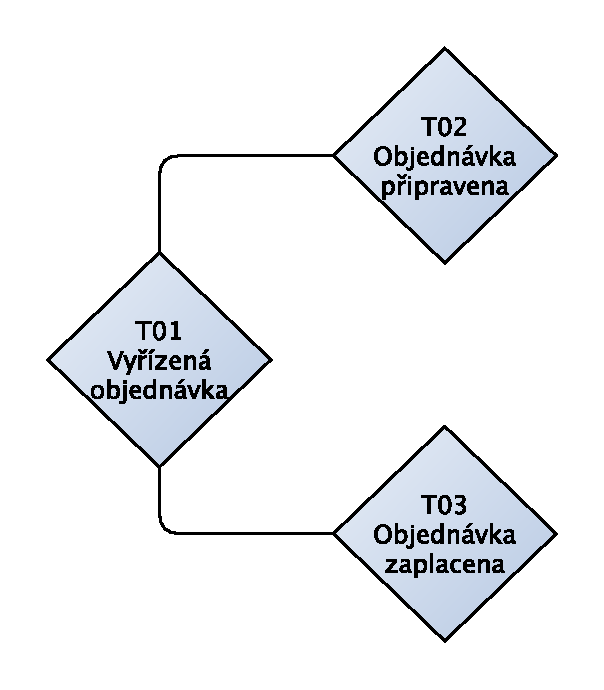
\includegraphics[scale=0.75]{obrazky/result-structure-chart-pizzeria}
\caption{Struktura závislosti transakcí v případu Pizzerie Mama Mia}
\label{fig:result_structure_chart}
\end{figure}

\subsection{Krok 6: Vytvoření DEMO modelů}
V předposledním kroku navržené metody je nutné vytvořit dva DEMO modely. Tyto modely slouží zejména pro zpětnou verifikaci vzniklého BPMN modelu.

Prvním vytvořeným modelem je Actor-Transaction Diagram (ATD), který zachycuje pouze transakce a actory, kteří se transakce účastní. Na obrázku \ref{fig:atd_pizzeria} můžeme vidět ATD pro případ Pizzerie Mama Mia. Zákazníka zde reprezentuje actor CA01 a jako jediný je vně organizace Pizzeria. Dalším actorem je Mia, která v tomto ATD vystupuje pod označením A01 a Mario, který je označen jako A02.

\begin{figure}[H]\centering
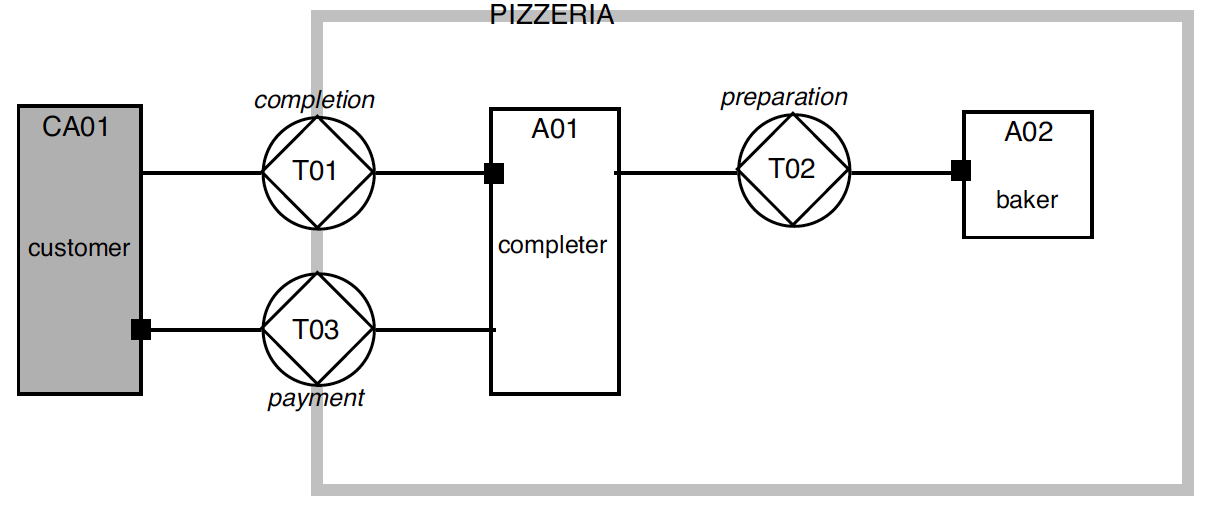
\includegraphics[scale=0.35]{obrazky/ATD-pizzeria}
\caption{ATD Pizzerie Mama Mia \cite{Dietz2006}}
\label{fig:atd_pizzeria}
\end{figure}

Pro vytváření výsledného BPMN modelu nám však bude více nápomocný Process Structure Diagram (PSD), který zachycuje všechny transakční kroky dle transakčního vzoru. V kroku 7 bude naším úkolem tyto transakční kroky vyjádřené v PSD popsat pomocí BPMN primitiv, které jsou popsány v sekci \ref{sec:tr_vzor_ulohy_signaly}.

Na \ref{fig:psd_pizzeria} můžem vidět PSD pro případ Pizzerie Mama Mia. Za povšimnutí stojí zejména šipky s přerušovaným tělem, které vyjadřují závislost vykonání C-actu na vykonání C-actu v jiné transakci. Díky tomu lze vidět, že vykonání Request T03 je závislé na Accept T02 a Execution T01 je závislá na Accept T03. Převedeno do lidské řeči to znamená, že než můžeme požádat zákazníka o zaplacení objednávky, musíme jí nejdřív připravit a zákazník ji musí akceptovat a že než je objednávka vyřízena musí dojít k jejímu zaplacení. Toto zjištění nám pomůže při vytváření BPMN modelu určit pořadí aktivit, které budeme propjovat pomocí sekvenčních toků.

\begin{figure}[H]\centering
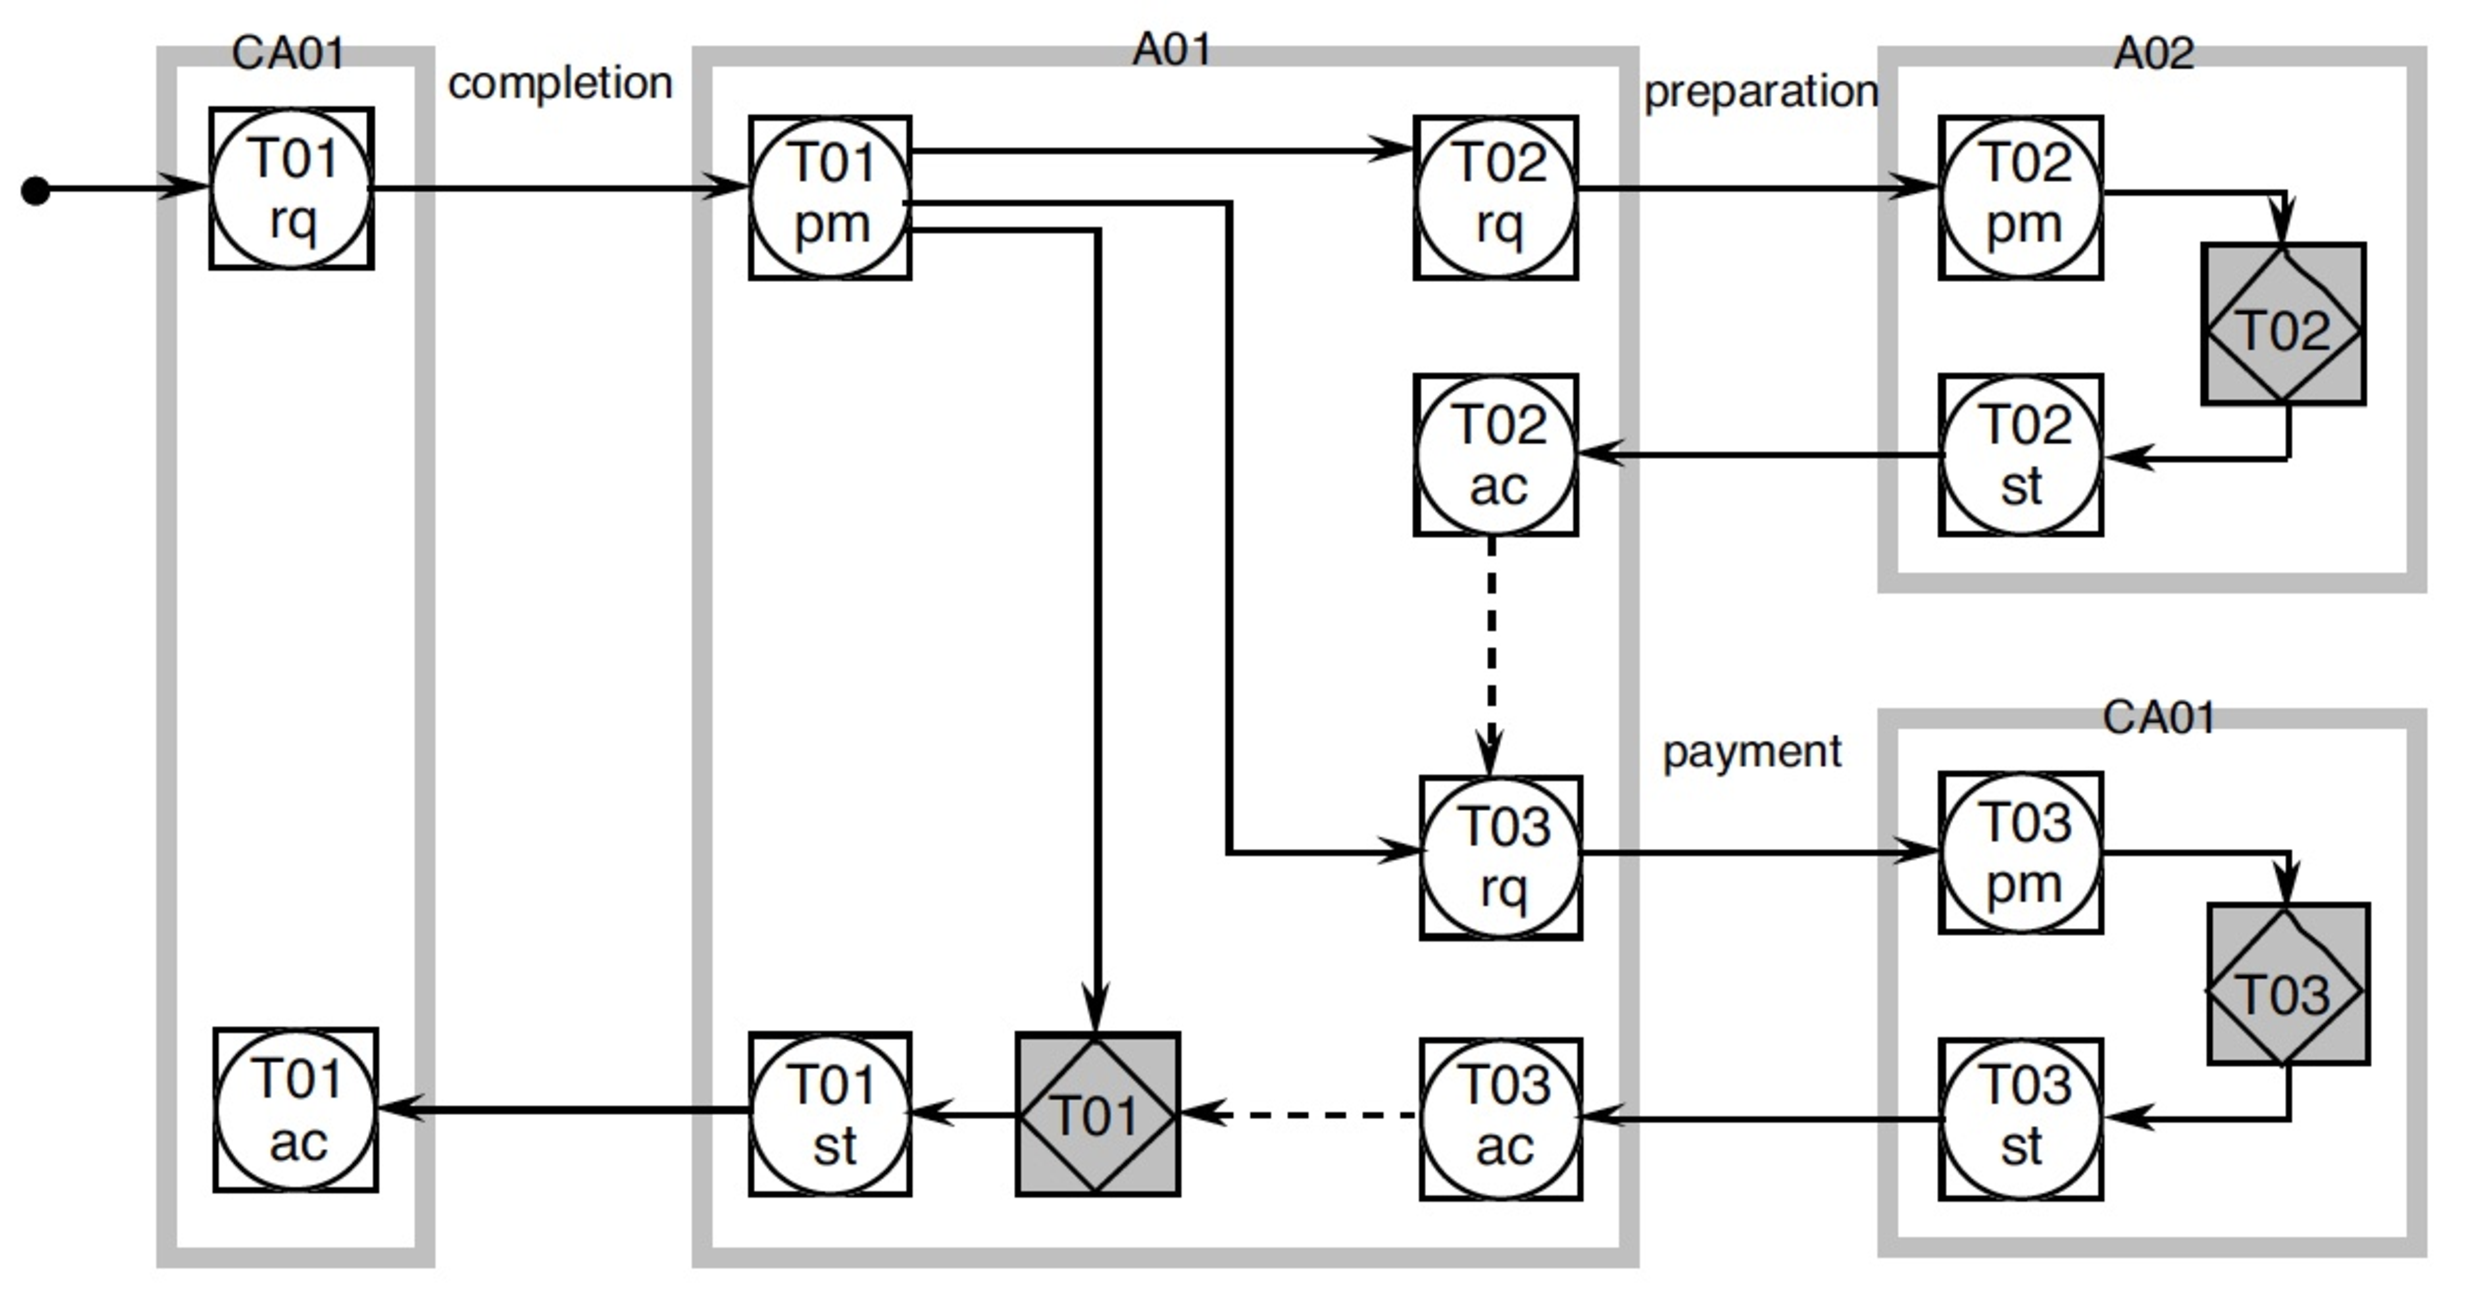
\includegraphics[scale=0.35]{obrazky/PSD-pizzeria}
\caption{PSD Pizzerie Mama Mia \cite{Dietz2006}}
\label{fig:psd_pizzeria}
\end{figure}

\subsection{Krok 7: Vytvoření BPMN modelu}
Nyní je vše připraveno pro vytvoření konečného BPMN modelu. Při jeho tvorbě budeme vycházet především z PSD modelu vytvořeného v předešlém kroce a z předpisu pro převedení transakčního axiomu do BPMN primitiv, který je uveden v sekci \ref{sec:tr_vzor_ulohy_signaly}. Postupujeme tedy po jednotlivých transakčních krocích zobrazených v PSD v obrázku \ref{fig:psd_pizzeria} a převádíme je dle tohoto předpisu do BPMN. Je důležité správně poskládat aktivity dle závislostí vyjádřených v kroku 5 i v PSD pomocí přerušovaných čar a diskutovaných v předchozím kroku.

Při vytváření PSD v předchozím kroku je použit pouze základní transakční vzor. Důvodem je větší čitelnost výsledného BPMN modelu a také absence popisu nešťastných scénářů v textovém popisu případu Pizzerie Mama Mia. Dle předpisu v sekci \ref{sec:tr_vzor_ulohy_signaly} by však nebyl problém vytvořit i BPMN model ze standardního transakčního vzoru.

Zobrazení případu Pizzerie Mama Mia v BPMN za použití metody navržené v této práci můžeme vidět na obrázku:

\begin{center}
\begin{figure}[H]
\centerline{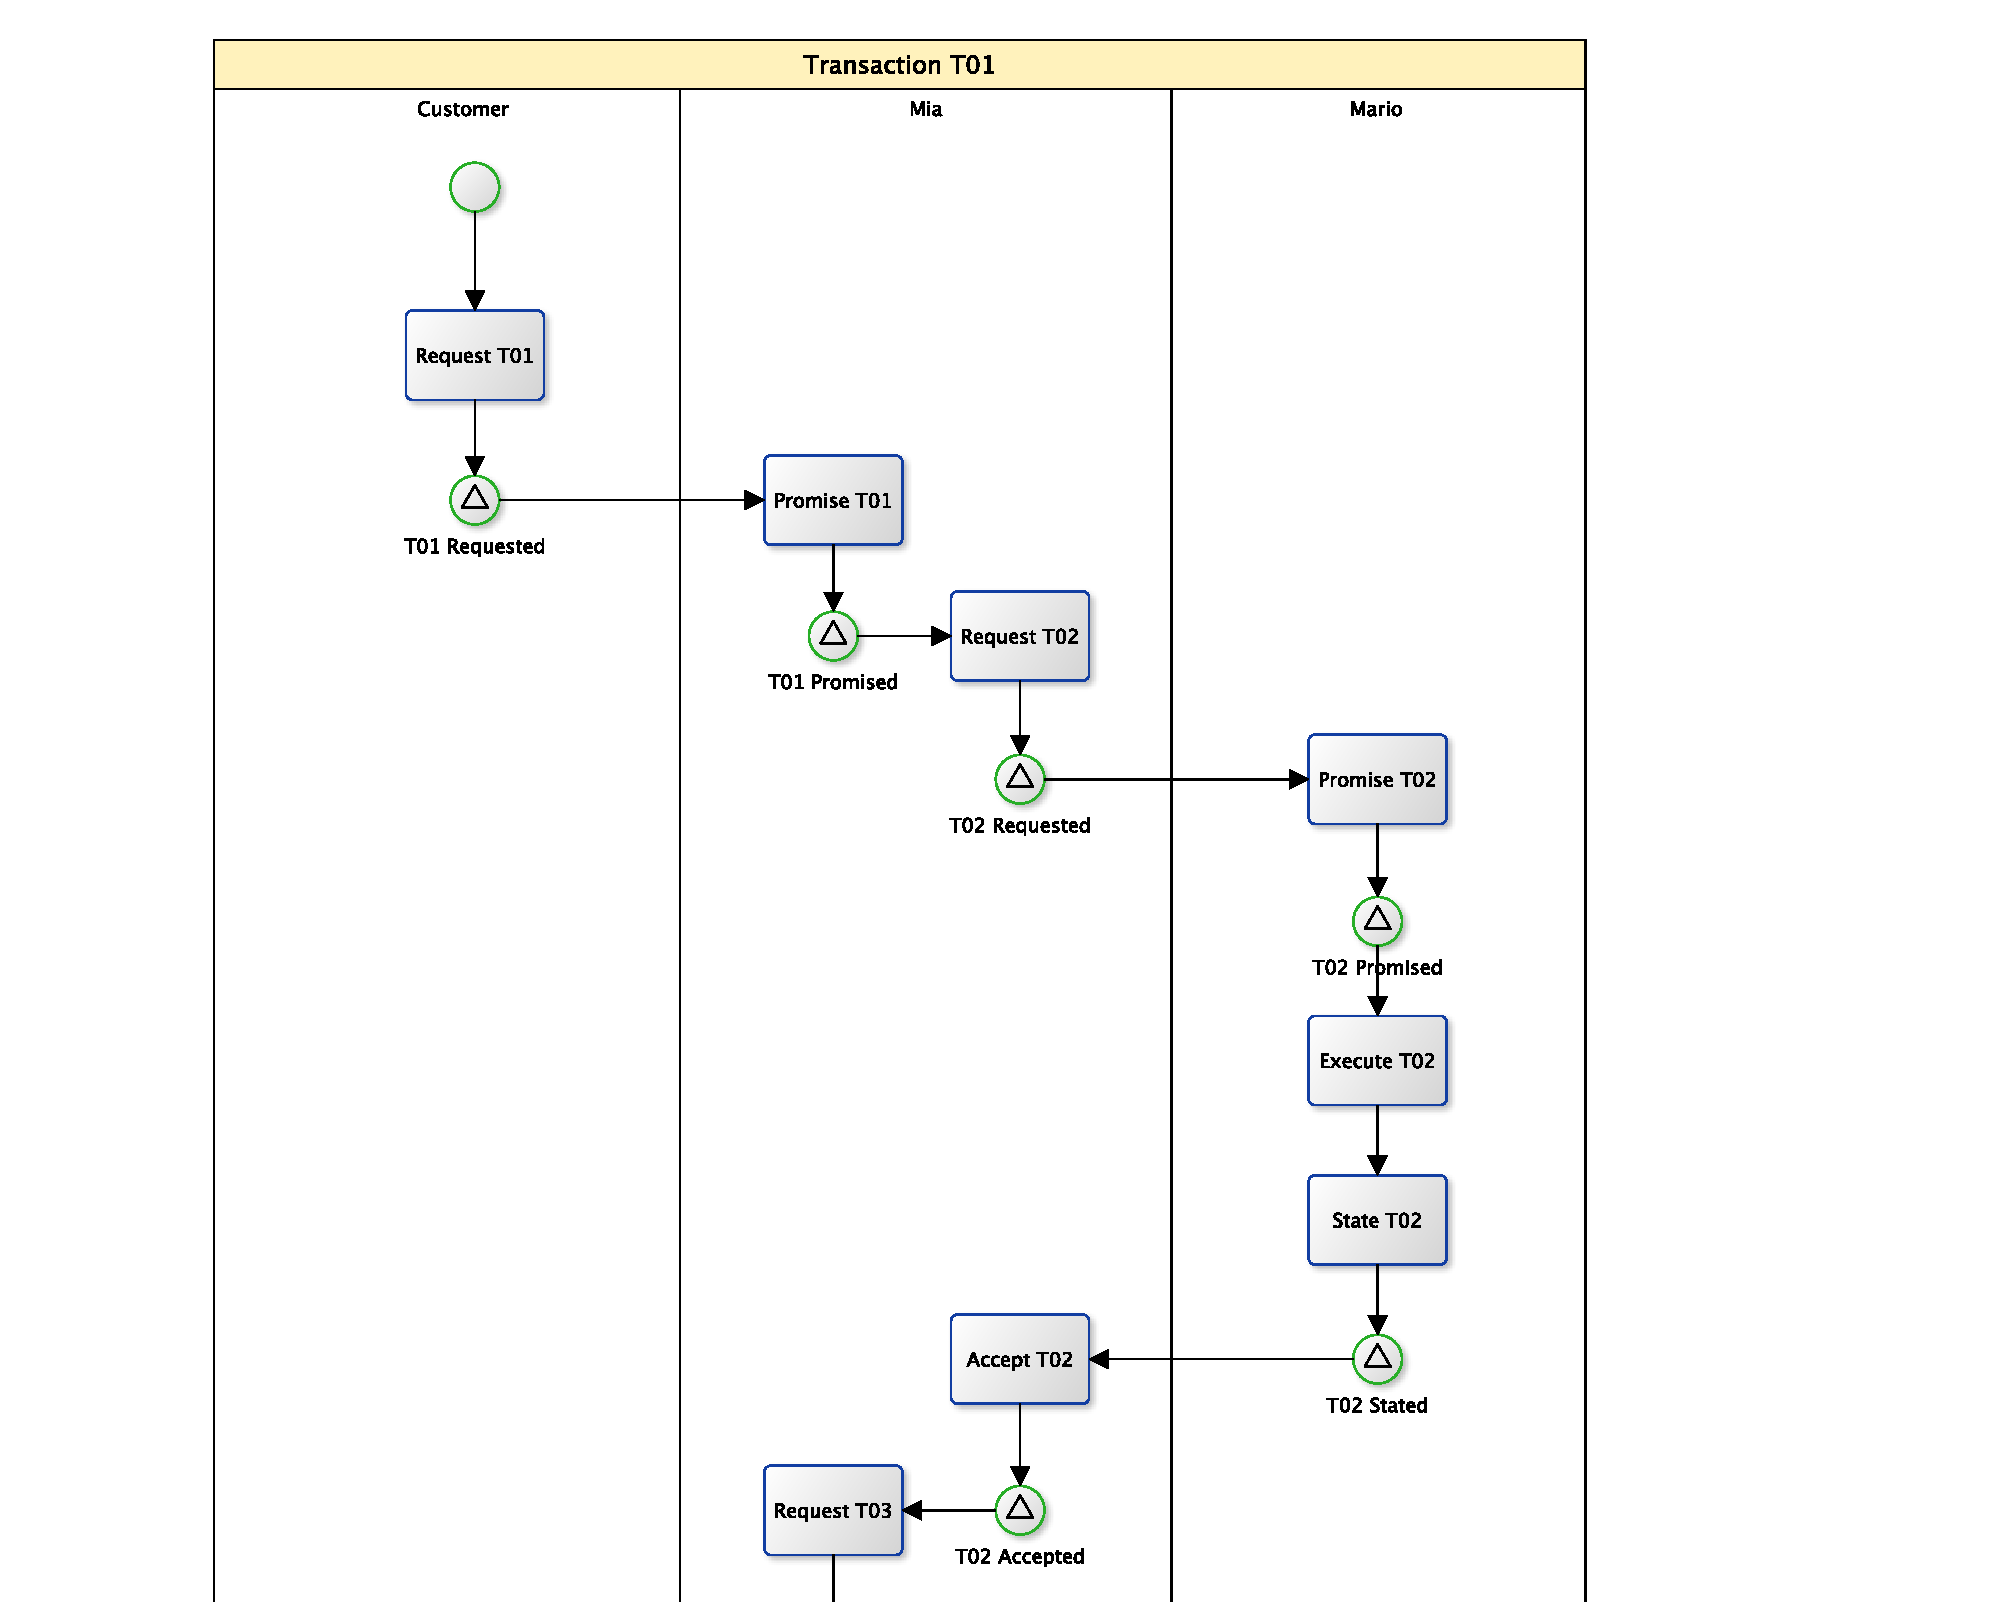
\includegraphics[width=1.28\textwidth,height=\textheight,keepaspectratio]{obrazky/pizzeria-bpmn-1}}
\caption{Případ Pizzerie Mama Mia v BPMN 1/2}
\label{fig:pizzeria_bpmn_1}
\end{figure}
\end{center}

\begin{center}
\begin{figure}[H]
\centerline{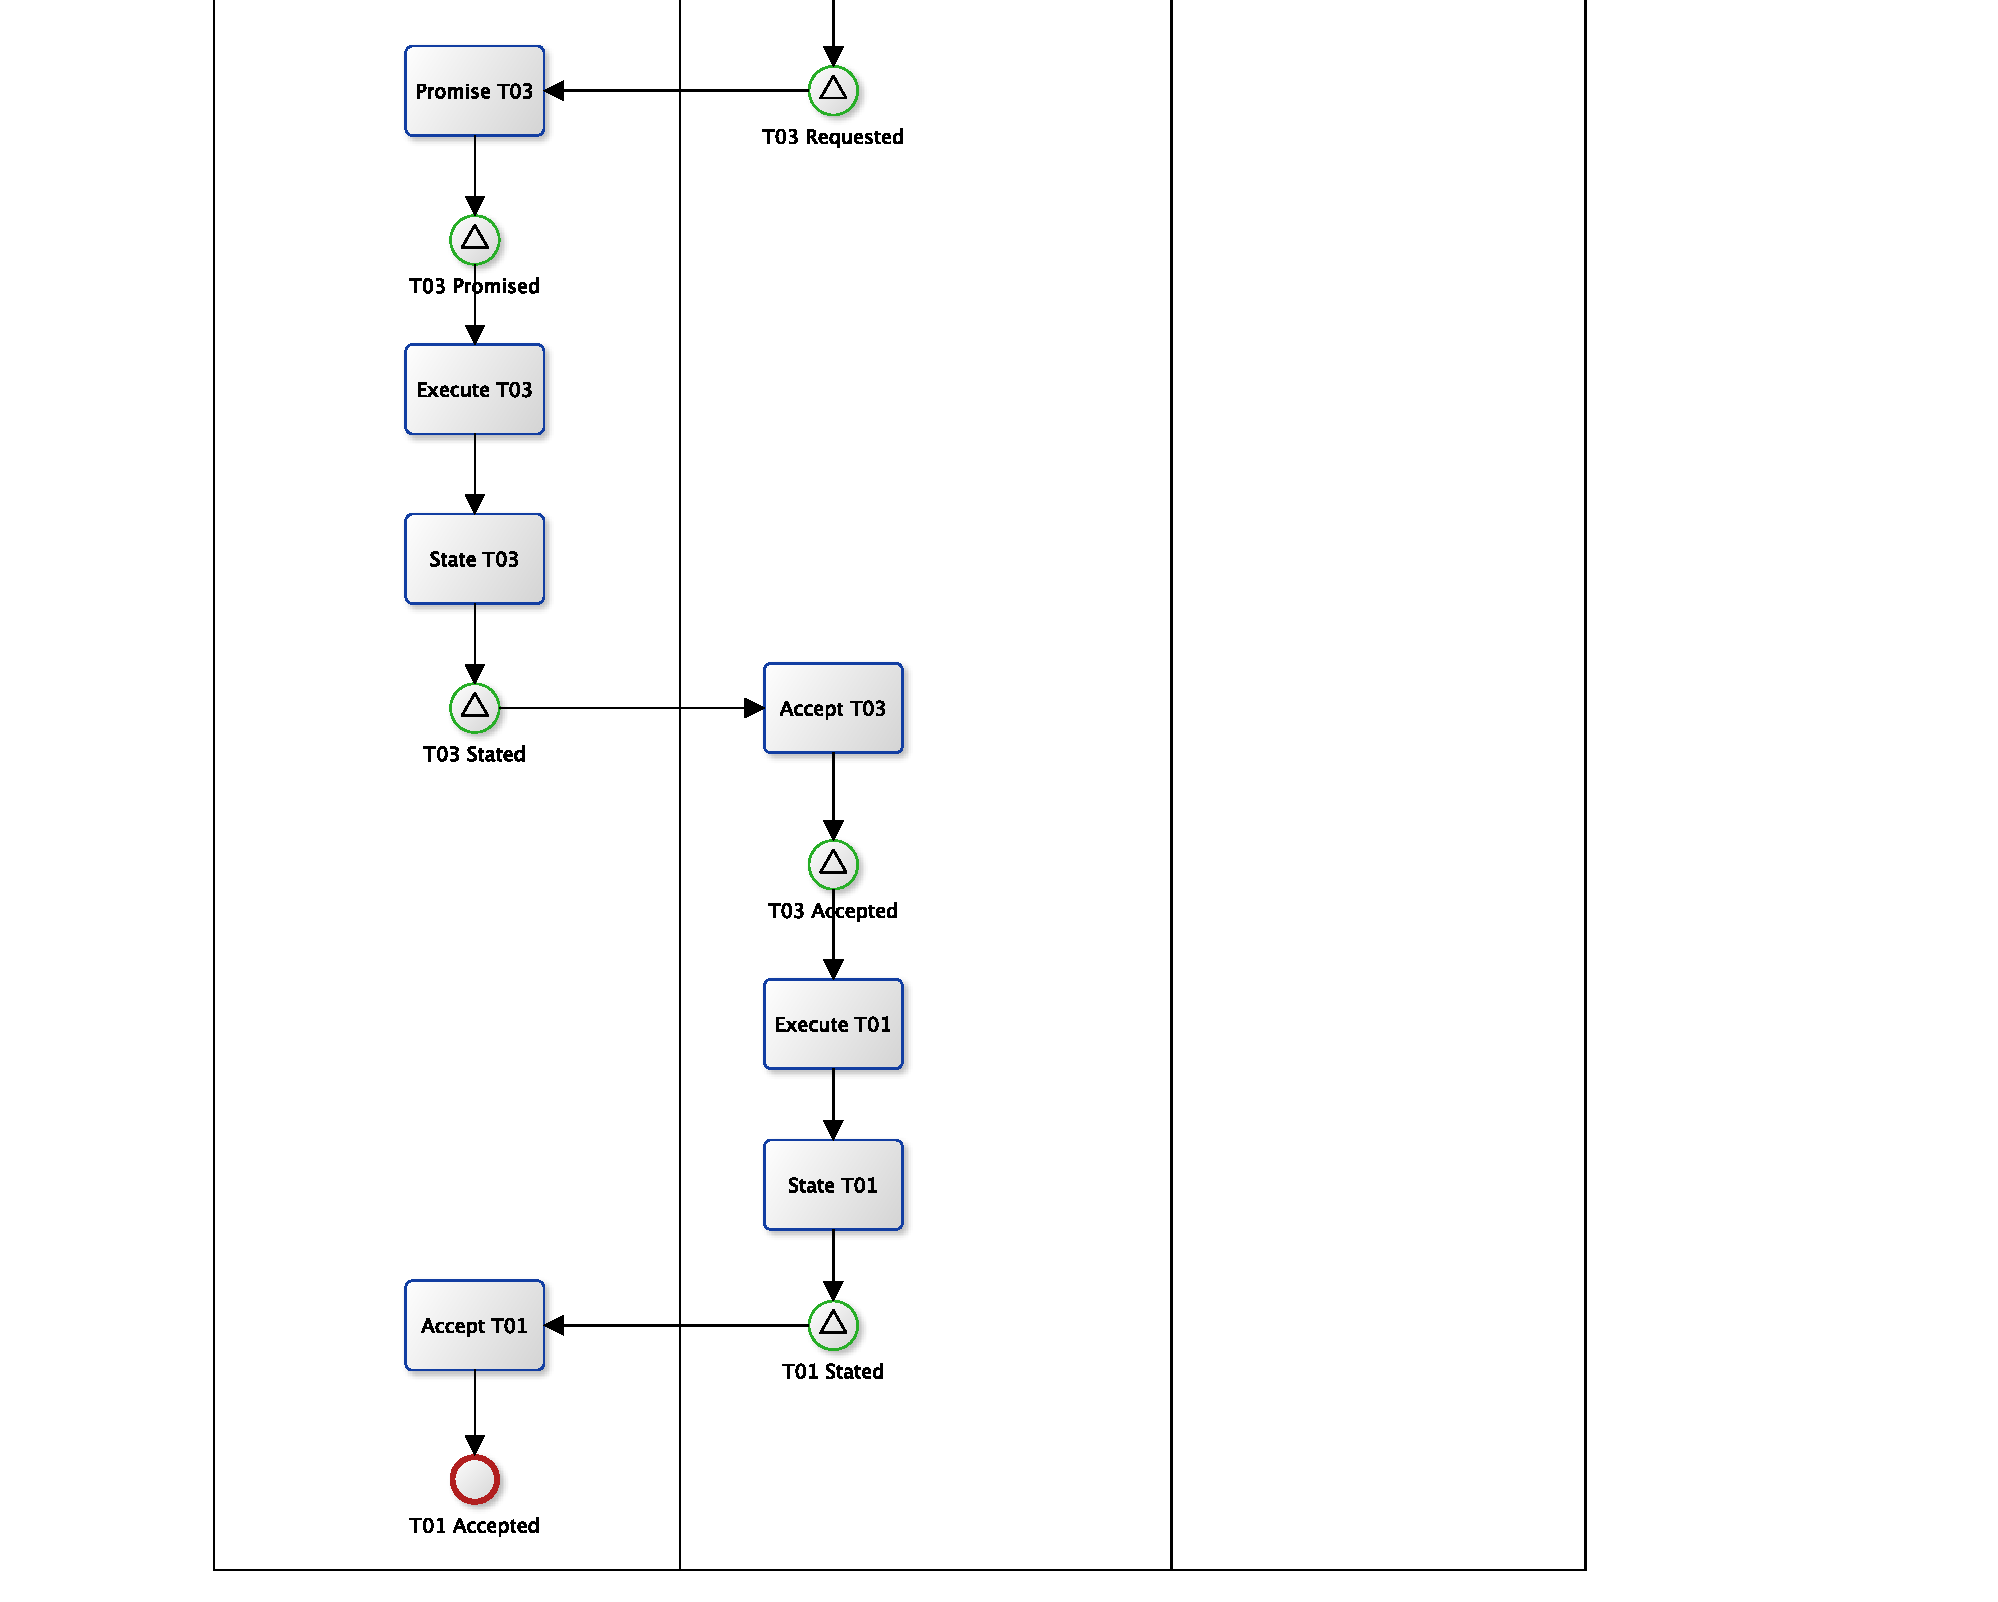
\includegraphics[width=1.28\textwidth,height=\textheight,keepaspectratio]{obrazky/pizzeria-bpmn-2}}
\caption{Případ Pizzerie Mama Mia v BPMN 2/2}
\label{fig:pizzeria_bpmn_2}
\end{figure}
\end{center}

\section{Diskuse}
Na obrázcích \ref{fig:pizzeria_bpmn_1} a \ref{fig:pizzeria_bpmn_2} vidíme, že se nám podařilo vytvořit BPMN model pro případ Pizzerie Mama Mia dle metody navržené v kapitole 5. Vytvořený BPMN model je:

\begin{itemize}
\item \textit{kompletní} dle transakčního axiomu – žádný transakční krok dle základního transakčního vzoru v modelu nechybí a díky použití plaveckých drah je jasné, který actor je zodpovědný za vykonání konkrétního transakčního kroku
\item \textit{konzistentní} dle transakčního axiomu – pořadí provádění všech transakčních kroků je konzistentní se základním transakčním vzorem
\item \textit{jednoznačný} – navržená metoda zajišťuje, že při správném aplikování všech kroků metody vznikne vždy ten samý model
\item \textit{esenciální} – výsledný model neobsahuje žádné implementační detaily. Při jeho tvorbě bylo použito pouze aktivit, které jsme vyhodnotili jako Performa.
\end{itemize}

\subsection{Slabiny metody}
\subsubsection{Modelování komplexních procesů}
Na obrázcích \ref{fig:pizzeria_bpmn_1} a \ref{fig:pizzeria_bpmn_2} jsou zachyceny pouze 3 transakce za použití základního transakčního vzoru a stejně jsme museli diagram rozdělit na 2 obrázky, protože se celý nevešel na jednu stránku. V případě modelování komplexnějších procesů, které obsahují desítky transakcí bude problém jen narůstat a model se bude obtížně vytvářet i číst.

Řešením je v tomto případě automatické generování BPMN diagramu z ATD diagramu (případně PSD dle DEMO 3) , který je mnohem méně obsáhlý a dobře čitelný i když obsahuje desítky transakcí. Pokud by bylo možné automatizovat vytváření BPMN a jejich verifikaci dle DEMO modelů, jednalo by se o velký krok dopředu.

\subsubsection{Korektní provedení kroku 2}
Z mé zkušenosti je pro velké množství lidí velmi problematické správně aplikovat krok 2 navržené metody, neboli správně provést na textovém popisu procesu Performa-Informa-Forma analýzu. Lidská řeč je totiž velmi vágní a rozdíly mezi Performa, Informa i Forma aktivitami jsou často nezřetelné a ani odborníkům se zkušenostmi s DEMO se často nedaří provést tento krok správně.

Na tomto místě je třeba uvést, že i situace, kdy se nepodaří všechny aktivity správně zařadit a jako Performa je napříkad zařazena aktivita, která Performa není, stále pravděpodobně vznikne kvalitnější BPMN model než by vzniknul neaplikováním této metody. Jak popisuje \cite{Silver2011} \uv{špatné BPMN} je dnes spíše pravidlem než výjimkou a aplikace navržené metody by tedy za každých okolností přispěla obecně k lepším výsledkům.

\nocite{*}
\bibliographystyle{plain}
\bibliography{Bibliography}

\end{document}
	
\begin{conclusion}
	%sem napište závěr Vaší práce
\end{conclusion}

\nocite{*}
\bibliographystyle{csn690}
\bibliography{Bibliography}

\appendix

\chapter{Seznam použitých zkratek}
% \printglossaries
\begin{description}
	\item[GUI] Graphical user interface
	\item[XML] Extensible markup language
\end{description}


% % % % % % % % % % % % % % % % % % % % % % % % % % % % 
% % Tuto kapitolu z výsledné práce ODSTRAŇTE.
% % % % % % % % % % % % % % % % % % % % % % % % % % % % 
% 
% \chapter{Návod k~použití této šablony}
% 
% Tento dokument slouží jako základ pro napsání závěrečné práce na Fakultě informačních technologií ČVUT v~Praze.
% 
% \section{Výběr základu}
% 
% Vyberte si šablonu podle druhu práce (bakalářská, diplomová), jazyka (čeština, angličtina) a kódování (ASCII, \mbox{UTF-8}, \mbox{ISO-8859-2} neboli latin2 a nebo \mbox{Windows-1250}). 
% 
% V~české variantě naleznete šablony v~souborech pojmenovaných ve formátu práce\_kódování.tex. Typ může být:
% \begin{description}
% 	\item[BP] bakalářská práce,
% 	\item[DP] diplomová (magisterská) práce.
% \end{description}
% Kódování, ve kterém chcete psát, může být:
% \begin{description}
% 	\item[UTF-8] kódování Unicode,
% 	\item[ISO-8859-2] latin2,
% 	\item[Windows-1250] znaková sada 1250 Windows.
% \end{description}
% V~případě nejistoty ohledně kódování doporučujeme následující postup:
% \begin{enumerate}
% 	\item Otevřete šablony pro kódování UTF-8 v~editoru prostého textu, který chcete pro psaní práce použít -- pokud můžete texty s~diakritikou normálně přečíst, použijte tuto šablonu.
% 	\item V~opačném případě postupujte dále podle toho, jaký operační systém používáte:
% 	\begin{itemize}
% 		\item v~případě Windows použijte šablonu pro kódování \mbox{Windows-1250},
% 		\item jinak zkuste použít šablonu pro kódování \mbox{ISO-8859-2}.
% 	\end{itemize}
% \end{enumerate}
% 
% 
% V~anglické variantě jsou šablony pojmenované podle typu práce, možnosti jsou:
% \begin{description}
% 	\item[bachelors] bakalářská práce,
% 	\item[masters] diplomová (magisterská) práce.
% \end{description}
% 
% \section{Použití šablony}
% 
% Šablona je určena pro zpracování systémem \LaTeXe{}. Text je možné psát v~textovém editoru jako prostý text, lze však také využít specializovaný editor pro \LaTeX{}, např. Kile.
% 
% Pro získání tisknutelného výstupu z~takto vytvořeného souboru použijte příkaz \verb|pdflatex|, kterému předáte cestu k~souboru jako parametr. Vhodný editor pro \LaTeX{} toto udělá za Vás. \verb|pdfcslatex| ani \verb|cslatex| \emph{nebudou} s~těmito šablonami fungovat.
% 
% Více informací o~použití systému \LaTeX{} najdete např. v~\cite{wikilatex}.
% 
% \subsection{Typografie}
% 
% Při psaní dodržujte typografické konvence zvoleného jazyka. České \uv{uvozovky} zapisujte použitím příkazu \verb|\uv|, kterému v~parametru předáte text, jenž má být v~uvozovkách. Anglické otevírací uvozovky se v~\LaTeX{}u zadávají jako dva zpětné apostrofy, uzavírací uvozovky jako dva apostrofy. Často chybně uváděný symbol "{} (palce) nemá s~uvozovkami nic společného.
% 
% Dále je třeba zabránit zalomení řádky mezi některými slovy, v~češtině např. za jednopísmennými předložkami a spojkami (vyjma \uv{a}). To docílíte vložením pružné nezalomitelné mezery -- znakem \texttt{\textasciitilde}. V~tomto případě to není třeba dělat ručně, lze použít program \verb|vlna|.
% 
% Více o~typografii viz \cite{kobltypo}.
% 
% \subsection{Obrázky}
% 
% Pro umožnění vkládání obrázků je vhodné použít balíček \verb|graphicx|, samotné vložení se provede příkazem \verb|\includegraphics|. Takto je možné vkládat obrázky ve formátu PDF, PNG a JPEG jestliže používáte pdf\LaTeX{} nebo ve formátu EPS jestliže používáte \LaTeX{}. Doporučujeme preferovat vektorové obrázky před rastrovými (vyjma fotografií).
% 
% \subsubsection{Získání vhodného formátu}
% 
% Pro získání vektorových formátů PDF nebo EPS z~jiných lze použít některý z~vektorových grafických editorů. Pro převod rastrového obrázku na vektorový lze použít rasterizaci, kterou mnohé editory zvládají (např. Inkscape). Pro konverze lze použít též nástroje pro dávkové zpracování běžně dodávané s~\LaTeX{}em, např. \verb|epstopdf|.
% 
% \subsubsection{Plovoucí prostředí}
% 
% Příkazem \verb|\includegraphics| lze obrázky vkládat přímo, doporučujeme však použít plovoucí prostředí, konkrétně \verb|figure|. Například obrázek \ref{fig:float} byl vložen tímto způsobem. Vůbec přitom nevadí, když je obrázek umístěn jinde, než bylo původně zamýšleno -- je tomu tak hlavně kvůli dodržení typografických konvencí. Namísto vynucování konkrétní pozice obrázku doporučujeme používat odkazování z~textu (dvojice příkazů \verb|\label| a \verb|\ref|).
% 
% \begin{figure}\centering
% 	
\includegraphics[width=0.5\textwidth, angle=30]{cvut-logo-bw}
% 	\caption[Příklad obrázku]{Ukázkový obrázek v~plovoucím prostředí}\label{fig:float}
% \end{figure}
% 
% \subsubsection{Verze obrázků}
% 
% % Gnuplot BW i barevně
% Může se hodit mít více verzí stejného obrázku, např. pro barevný či černobílý tisk a nebo pro prezentaci. S~pomocí některých nástrojů na generování grafiky je to snadné.
% 
% Máte-li například graf vytvořený v programu Gnuplot, můžete jeho černobílou variantu (viz obr. \ref{fig:gnuplot-bw}) vytvořit parametrem \verb|monochrome dashed| příkazu \verb|set term|. Barevnou variantu (viz obr. \ref{fig:gnuplot-col}) vhodnou na prezentace lze vytvořit parametrem \verb|colour solid|.
% 
% \begin{figure}\centering
% 	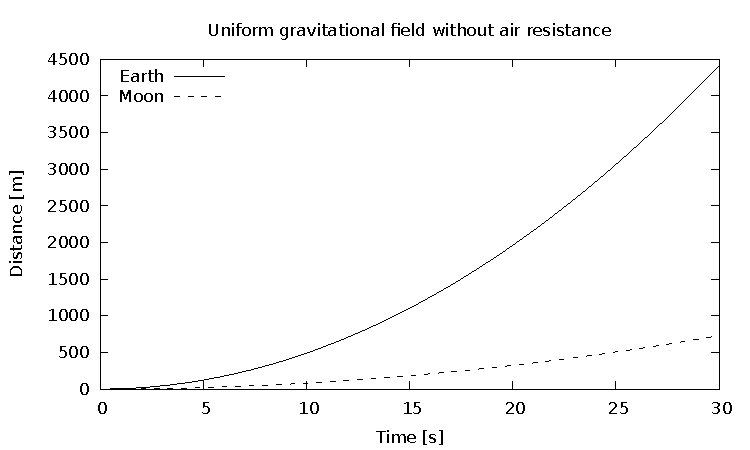
\includegraphics{gnuplot-bw}
% 	\caption{Černobílá varianta obrázku generovaného programem Gnuplot}\label{fig:gnuplot-bw}
% \end{figure}
% 
% \begin{figure}\centering
% 	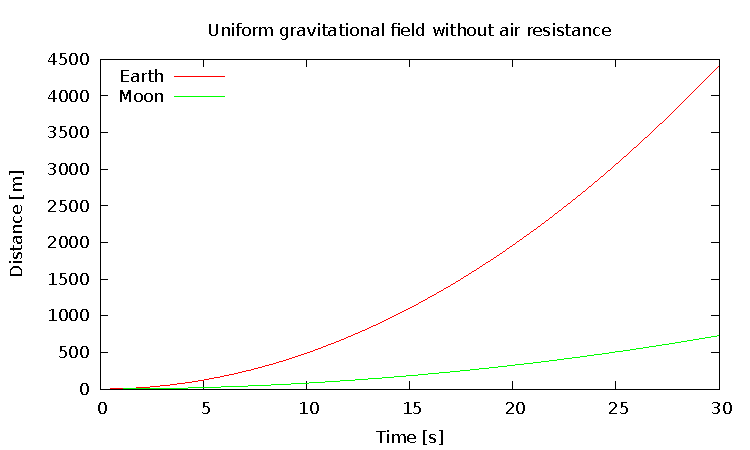
\includegraphics{gnuplot-col}
% 	\caption{Barevná varianta obrázku generovaného programem Gnuplot}\label{fig:gnuplot-col}
% \end{figure}
% 
% 
% \subsection{Tabulky}
% 
% Tabulky lze zadávat různě, např. v~prostředí \verb|tabular|, avšak pro jejich vkládání platí to samé, co pro obrázky -- použijte plovoucí prostředí, v~tomto případě \verb|table|. Například tabulka \ref{tab:matematika} byla vložena tímto způsobem.
% 
% \begin{table}\centering
% 	\caption[Příklad tabulky]{Zadávání matematiky}\label{tab:matematika}
% 	\begin{tabular}{|l|l|c|c|}\hline
% 		Typ		& Prostředí		& \LaTeX{}ovská zkratka	& \TeX{}ovská zkratka	\tabularnewline \hline \hline
% 		Text		& \verb|math|		& \verb|\(...\)|	& \verb|$...$|		\tabularnewline \hline
% 		Displayed	& \verb|displaymath|	& \verb|\[...\]|	& \verb|$$...$$|	\tabularnewline \hline
% 	\end{tabular}
% \end{table}
% 
% % % % % % % % % % % % % % % % % % % % % % % % % % % % 

\chapter{Obsah přiloženého CD}

%upravte podle skutecnosti

\begin{figure}
	\dirtree{%
		.1 readme.txt\DTcomment{stručný popis obsahu CD}.
		.1 exe\DTcomment{adresář se spustitelnou formou implementace}.
		.1 src.
		.2 impl\DTcomment{zdrojové kódy implementace}.
		.2 thesis\DTcomment{zdrojová forma práce ve formátu \LaTeX{}}.
		.1 text\DTcomment{text práce}.
		.2 thesis.pdf\DTcomment{text práce ve formátu PDF}.
		.2 thesis.ps\DTcomment{text práce ve formátu PS}.
	}
\end{figure}

\end{document}
